%%=============================================================================
%% Resultaten details
%%=============================================================================

\chapter{Details van resultaten}
\label{ch:details-van-resultaten}

\newpage

\section{Document 1}

\begin{figure}[H]
    \centering
    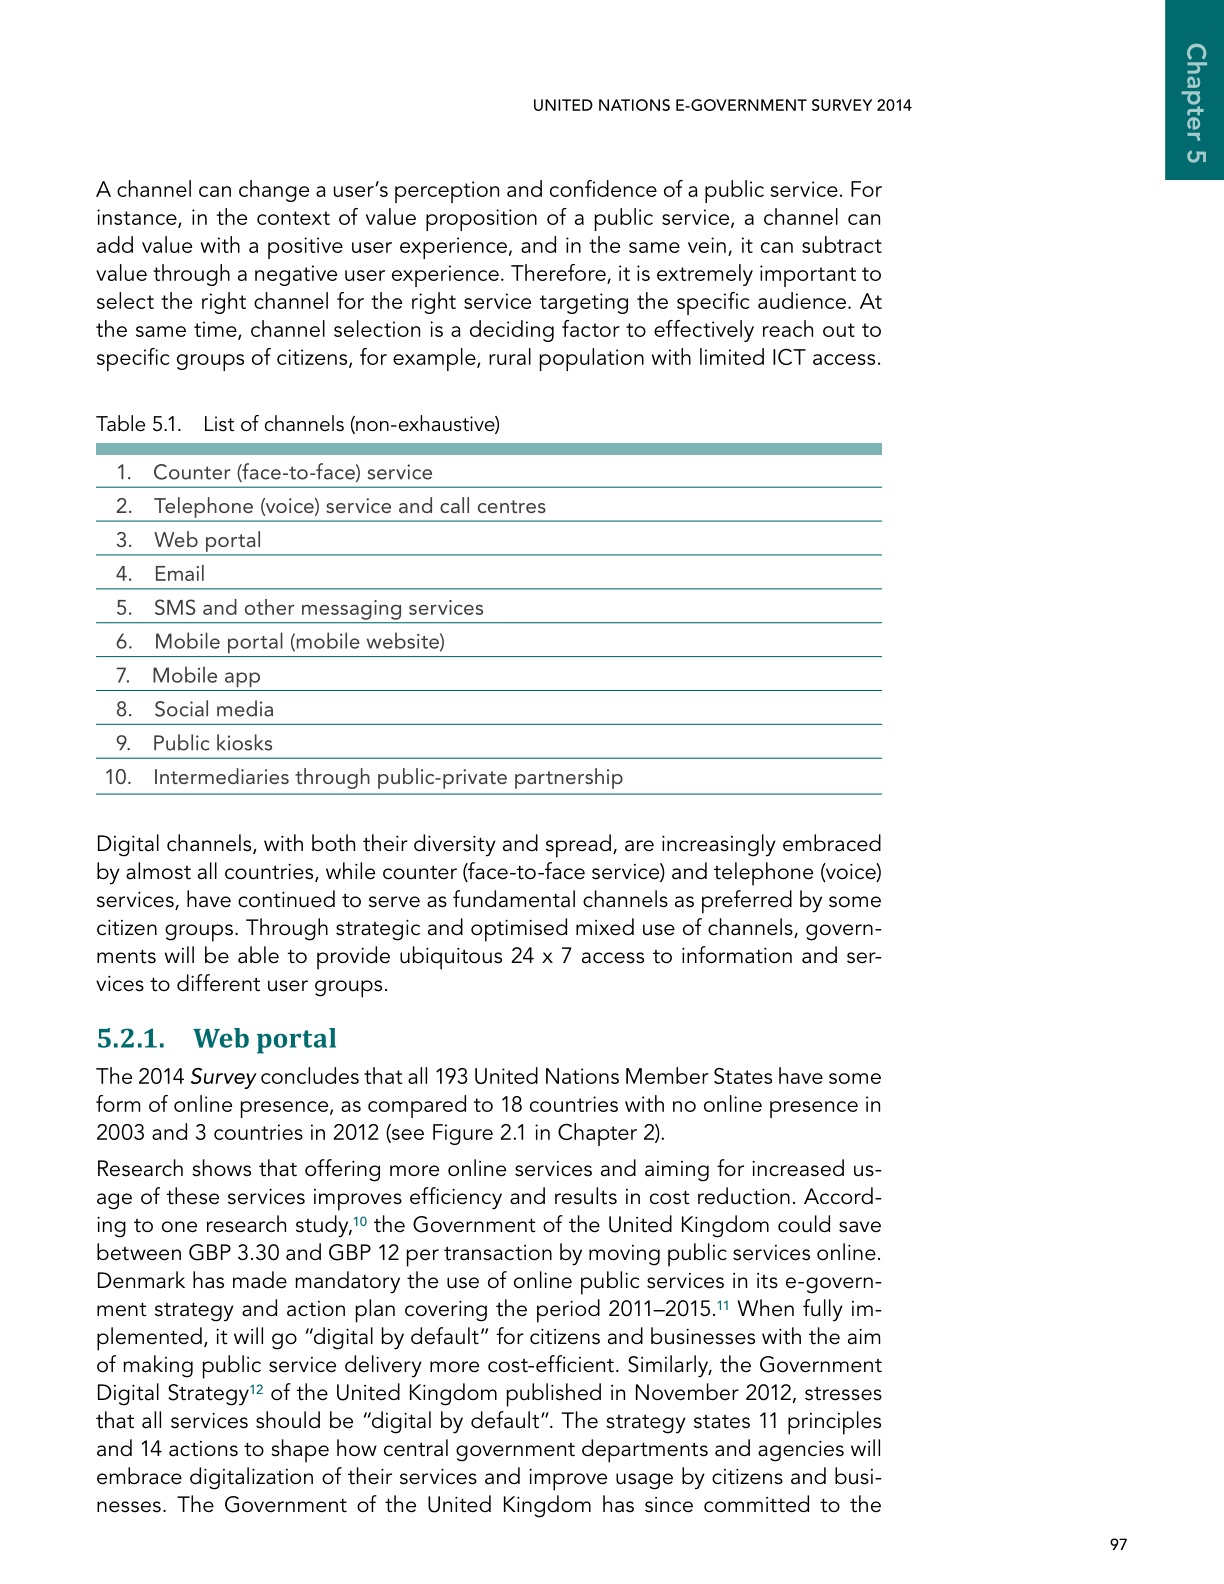
\includegraphics[width=0.8\textwidth]{test-resultaten/1/original.jpg}
    \caption{Origineel document.}
\end{figure}

\begin{figure}[H]
    \centering
    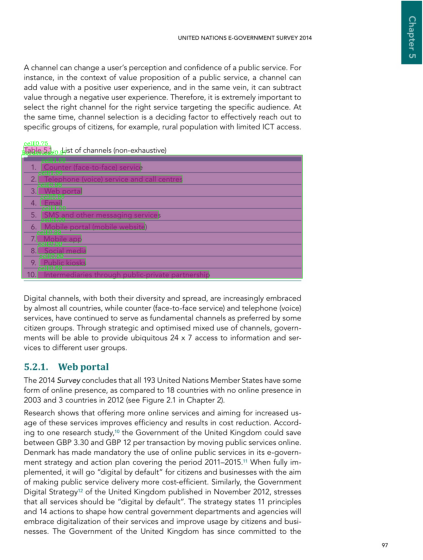
\includegraphics[width=0.8\textwidth]{test-resultaten/1/detected_tables.png}
    \caption{Gedetecteerde tabellen.}
\end{figure}

Getransformeerde tabellen met algoritme A:

\begin{tabular}{ll}
\toprule
{} &                     Counter (face-to-face) service \\
\midrule
0 &         Telephone (voice) service and call centres \\
1 &                                         Web portal \\
2 &                                               Emai \\
3 &                   SMS and other messaging service: \\
4 &                      Mobile portal (mobile website \\
5 &                                      7. Mobile apo \\
6 &                                       Social media \\
7 &                                      Public kiosks \\
8 &  Intermediaries through public-private partnershir \\
\bottomrule
\end{tabular}

Getransformeerde tabellen met algoritme B:

\begin{tabular}{ll}
\toprule
{} &                  1. Counter (face-to-face) service \\
\midrule
0 &      2. Telephone (voice) service and call centres \\
1 &                                      3. Web portal \\
2 &                                           4. Email \\
3 &                5. SMS and other messaging services \\
4 &                  6. Mobile portal (mobile website) \\
5 &                                      7. Mobile app \\
6 &                                    8. Social media \\
7 &                                   9. Public kiosks \\
8 &  10. Intermediaries through public-private part... \\
\bottomrule
\end{tabular}

\section{Document 2}

\begin{figure}[H]
    \centering
    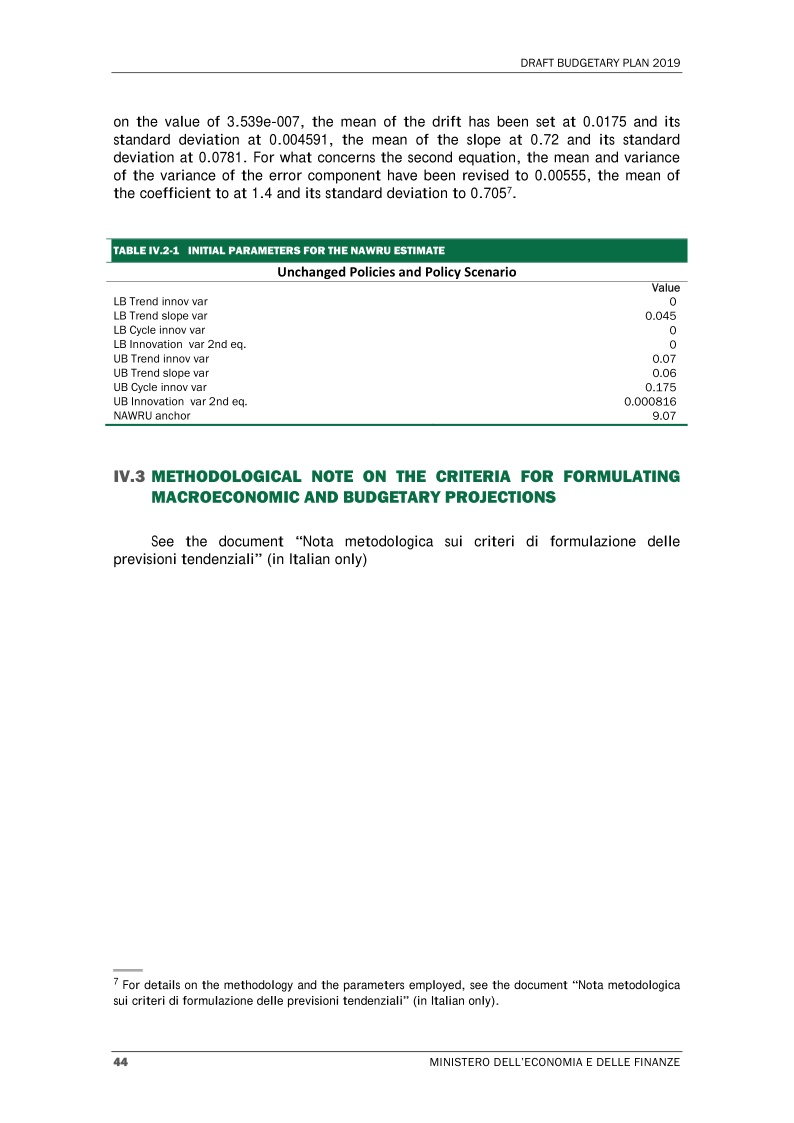
\includegraphics[width=0.8\textwidth]{test-resultaten/2/original.jpg}
    \caption{Origineel document.}
\end{figure}

\begin{figure}[H]
    \centering
    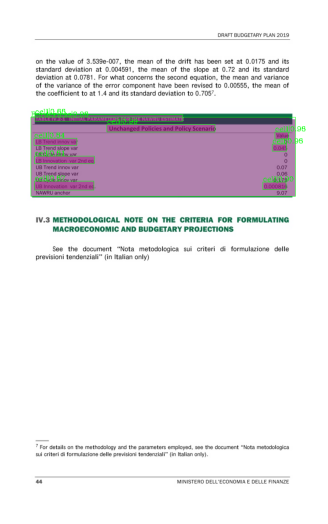
\includegraphics[width=0.8\textwidth]{test-resultaten/2/detected_tables.png}
    \caption{Gedetecteerde tabellen.}
\end{figure}

Getransformeerde tabellen met algoritme A:

Tabeltransformatie gefaald.

Getransformeerde tabellen met algoritme B:

\begin{tabular}{lll}
\toprule
{} &                      ate haath alee eid &       NaN \\
\midrule
0  &  Unchanged Policies and Policy Scenario &      None \\
1  &                                    None &      Vane \\
2  &                      L8 Trend innov var &        90 \\
3  &                      LB Trend slope var &     0.045 \\
4  &                       LB Cycle inno var &         0 \\
5  &               LB Innovation var 2nd ea, &         0 \\
6  &                      UB Trend Innov var &       O07 \\
7  &                      UB Trend stope var &      0.08 \\
8  &                      UB Cycle innov var &     0.178 \\
9  &               UB Innovation var 2nd ea, &  0.000816 \\
10 &                            NAWRU anchor &     ‘9.07 \\
\bottomrule
\end{tabular}
\section{Document 3}

\begin{figure}[H]
    \centering
    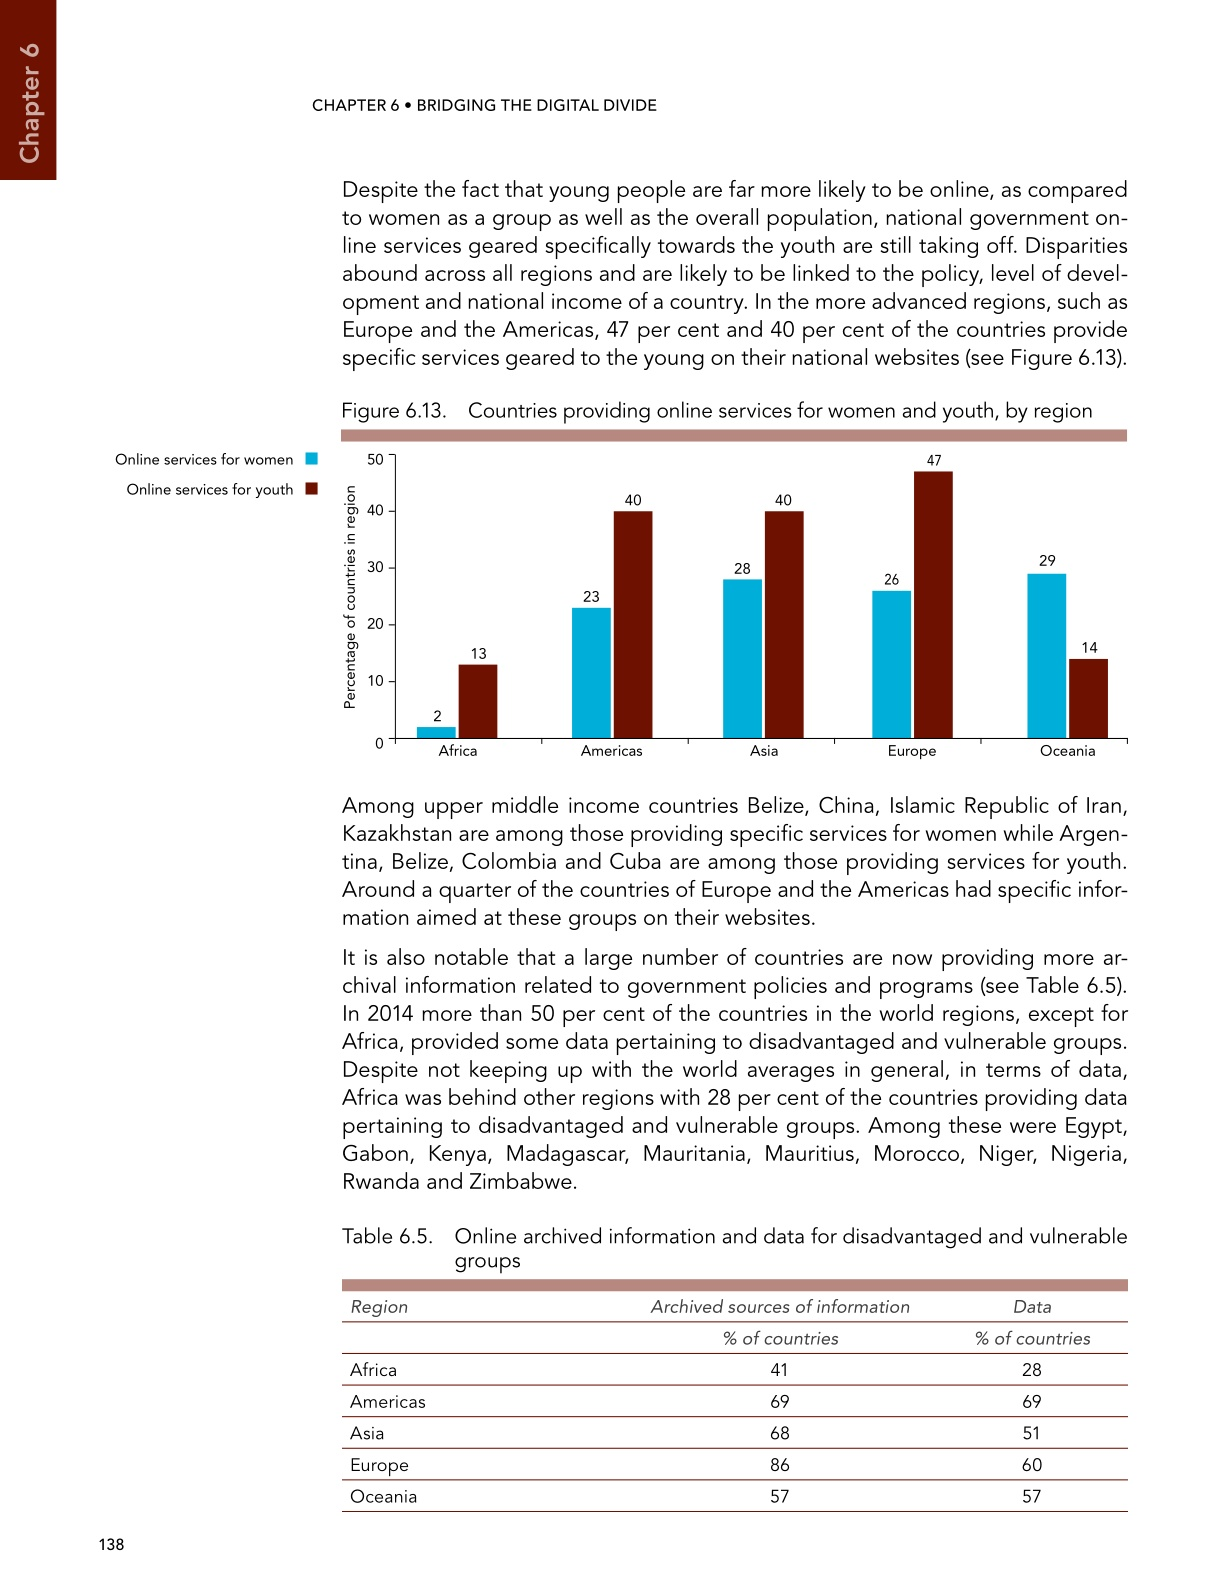
\includegraphics[width=0.8\textwidth]{test-resultaten/3/original.jpg}
    \caption{Origineel document.}
\end{figure}

\begin{figure}[H]
    \centering
    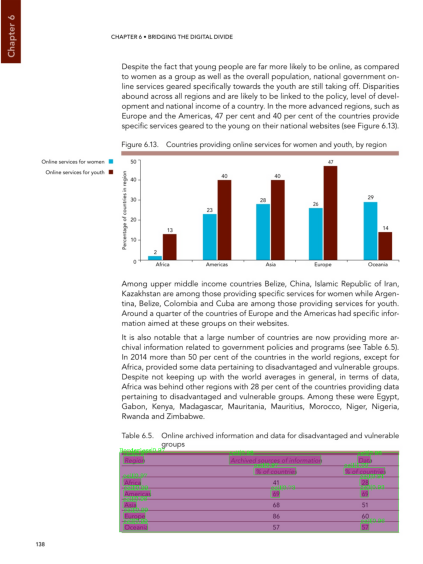
\includegraphics[width=0.8\textwidth]{test-resultaten/3/detected_tables.png}
    \caption{Gedetecteerde tabellen.}
\end{figure}

Getransformeerde tabellen met algoritme A:

\begin{tabular}{llll}
\toprule
{} &          Region & Archived sources of information &  Data \\
\midrule
0 &  \% of countries &                  \% of countries &  None \\
1 &          Africa &                              Al &    28 \\
2 &        Americas &                              69 &    69 \\
3 &            Asia &                              68 &    51 \\
4 &          Europe &                              Bb &    60 \\
5 &         Oceania &                              57 &    57 \\
\bottomrule
\end{tabular}

Getransformeerde tabellen met algoritme B:

\begin{tabular}{llll}
\toprule
{} &    Region & Archived sources of information &            Data \\
\midrule
0 &      None &                  \% of countries &  \% of countries \\
1 &    Africa &                               A &              28 \\
2 &  Americas &                              69 &              69 \\
3 &      Asia &                              68 &              51 \\
4 &    Europe &                              86 &              60 \\
5 &   Oceania &                              57 &              a7 \\
\bottomrule
\end{tabular}

\section{Document 4}

\begin{figure}[H]
    \centering
    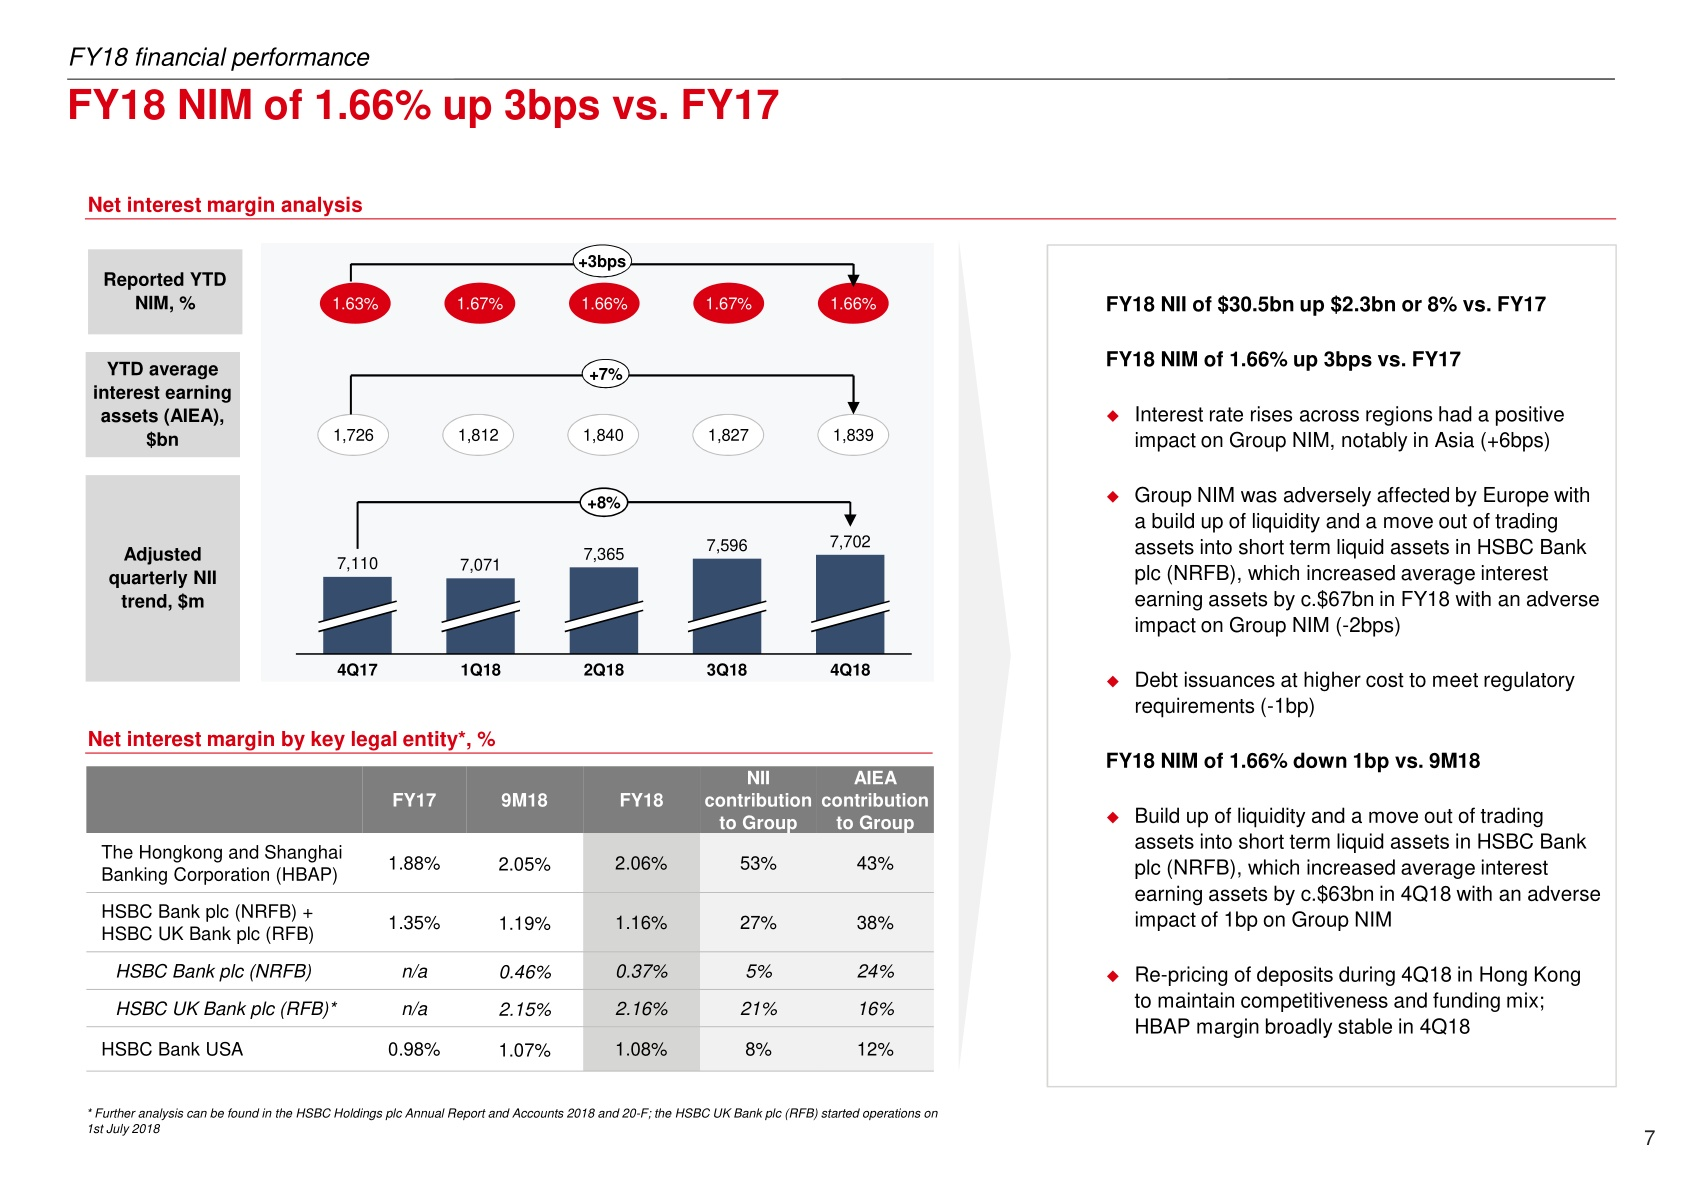
\includegraphics[width=0.8\textwidth]{test-resultaten/4/original.jpg}
    \caption{Origineel document.}
\end{figure}

\begin{figure}[H]
    \centering
    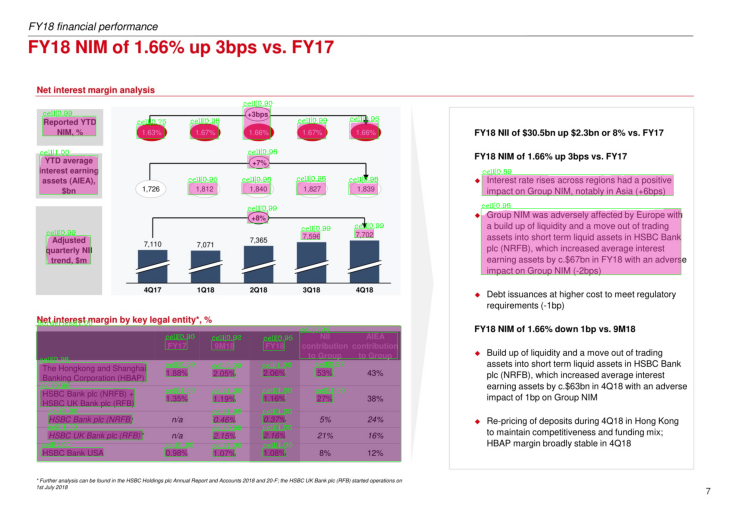
\includegraphics[width=0.8\textwidth]{test-resultaten/4/detected_tables.png}
    \caption{Gedetecteerde tabellen.}
\end{figure}

Getransformeerde tabellen met algoritme A:

Tabeltransformatie gefaald.

Getransformeerde tabellen met algoritme B:

\begin{tabular}{lllllll}
\toprule
{} &                      The Hongkong and Shanghai &  1.88\% &  2.05\% &  2.06\% &    53\% &      43\% \\
\midrule
0 &                     Banking Corporation (HBAP) &   None &   None &   None &   None &     None \\
1 &  HSBC Bank ple (NRFB) + HSBC UK Bank ple (RFB) &  1.35\% &  1.19\% &  1.16\% &    27\% &      38\% \\
2 &                           HSBC Bank plc (NRFB) &     Wa &  0.46\% &  0.37\% &     5\% &      24\% \\
3 &                        HSBC UK Bank plo (RFB)* &     na &  2.15\% &  2.16\% &    21\% &      16\% \\
4 &                                  HSBC Bank USA &  0.98\% &  1.07\% &  1.08\% &     8\% &      12\% \\
5 &                                           None &   FY17 &    ey) &    aly &   Pele &  mr hel) \\
6 &                                           None &   None &   None &   None &    ii\} &       rN \\
7 &                                           None &   None &   None &   None &  eect) &   feeds) \\
\bottomrule
\end{tabular}
\section{Document 5}

\begin{figure}[H]
    \centering
    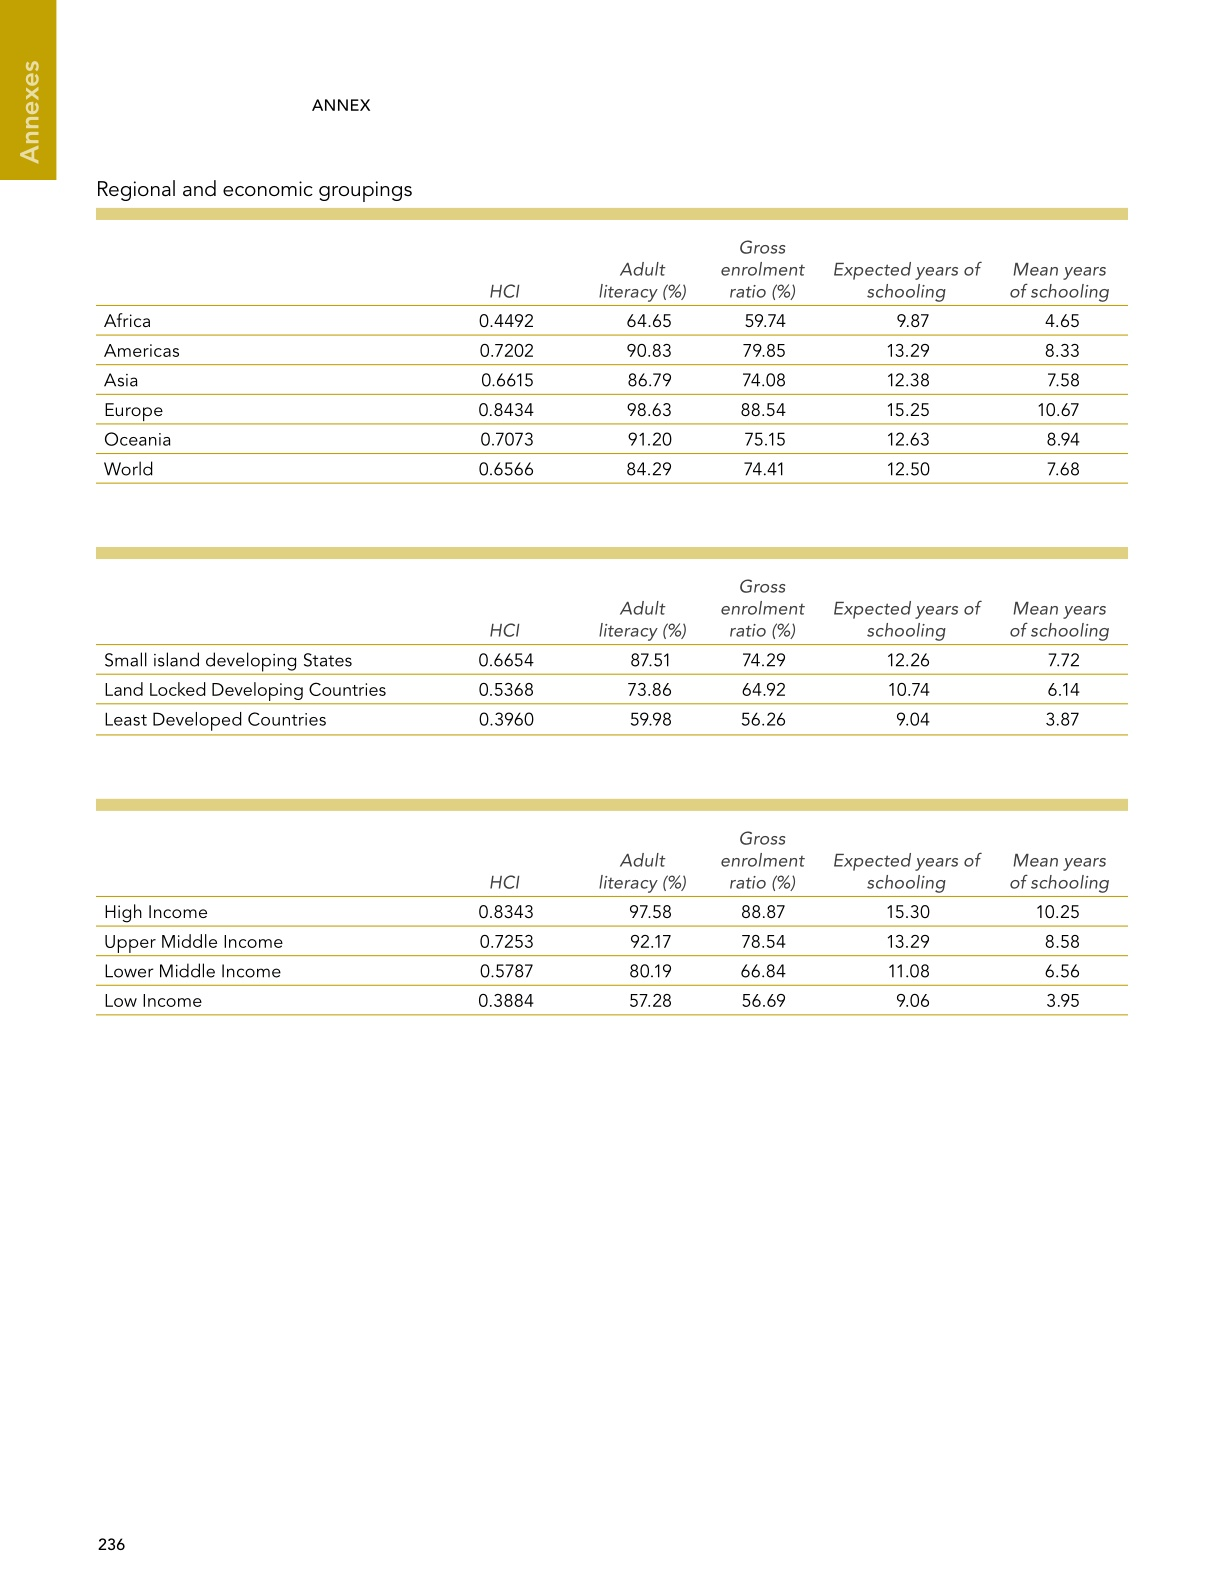
\includegraphics[width=0.8\textwidth]{test-resultaten/5/original.jpg}
    \caption{Origineel document.}
\end{figure}

\begin{figure}[H]
    \centering
    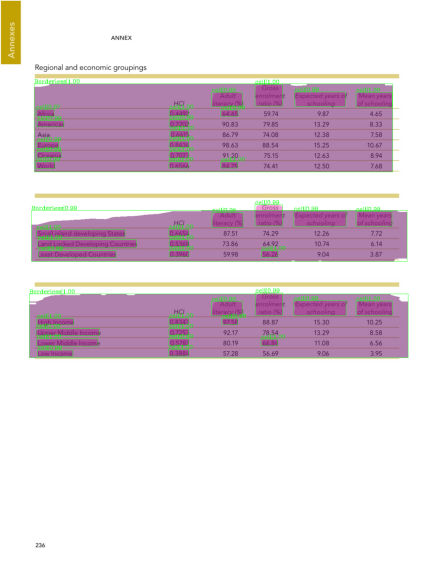
\includegraphics[width=0.8\textwidth]{test-resultaten/5/detected_tables.png}
    \caption{Gedetecteerde tabellen.}
\end{figure}

Getransformeerde tabellen met algoritme A:

\begin{tabular}{lllll}
\toprule
{} & Adult\textbackslash nliteracy (\% & Gross\textbackslash nenrolmen\textbackslash nratio (\%) & Expected years of\textbackslash nschooling & Mean years\textbackslash nof schooling \\
\midrule
0 &             Africa &                      59.74 &                          987 &                      465 \\
1 &           Americas &                      79.85 &                        13.29 &                     8.33 \\
2 &              06615 &                      74.08 &                        12.38 &                     7.58 \\
3 &             Europe &                      88.54 &                        15.25 &                    10.67 \\
4 &            Oceania &                      75.15 &                        12.63 &                      894 \\
5 &              World &                      74.41 &                        12.50 &                     7.68 \\
\bottomrule
\end{tabular}

\begin{tabular}{lllll}
\toprule
{} &  Adult\textbackslash nliteracy (\%, & Gross\textbackslash nenrolment\textbackslash nratio (\%) & Expected years of\textbackslash nschooling & Mean years\textbackslash nof schooling \\
\midrule
0 &          High Income &                       88.87 &                        15.30 &                    10.25 \\
1 &  Upper Middle Income &                       78.54 &                        13.29 &                     8.58 \\
2 &  Lower Middle Incom: &                       66.84 &                        11.08 &                     6.56 \\
3 &           Low Income &                       56.69 &                         9.06 &                      395 \\
\bottomrule
\end{tabular}

\begin{tabular}{lllll}
\toprule
{} &               Adult\textbackslash nliteracy (\%) & enrolment\textbackslash nratio (\%) & Expected years of\textbackslash nschooling & Mean years\textbackslash nof schooling \\
\midrule
0 &    Small island developing States &                74.29 &                        12.26 &                      772 \\
1 &  Land Locked Developing Countrie: &                64.92 &                        10.74 &                     6.14 \\
2 &         Least Developed Countries &                56.26 &                          904 &                       oF \\
\bottomrule
\end{tabular}

Getransformeerde tabellen met algoritme B:

\begin{tabular}{lllllll}
\toprule
{} &        Gross &           NaN &               NaN &           NaN &     NaN &       NaN \\
\midrule
0 &    enrolment &         Adult &  Expected yearsof &    Mean years &    None &      None \\
1 &  \_\_ratio (\%) &  literacy (\%) &         schooling &  of schooling &     HCI &      None \\
2 &        59.74 &         64.65 &              9.87 &          4.65 &  0.4492 &    Africa \\
3 &        79.85 &         90.83 &             13.29 &          8.33 &  0.7202 &  Americas \\
4 &        74.08 &         86.79 &             12.38 &          7.58 &  0.6615 &      Asia \\
5 &        88.54 &         98.63 &             18.25 &         10.67 &  0.8434 &    Europe \\
6 &        75.15 &         91.20 &             12.63 &          8.94 &  0.7073 &   Oceania \\
7 &         None &         84.29 &             12.50 &          7.68 &  0.6566 &     World \\
\bottomrule
\end{tabular}

\begin{tabular}{lllllll}
\toprule
{} &                     Gross &               NaN &           NaN &           NaN &     NaN &     NaN \\
\midrule
0 &           Adult enrolment &  Expected yearsof &    Mean years &          None &    None &    None \\
1 &  literacy (\%) \_ ratio (\%) &         schooling &  of schooling &          None &    None &    None \\
2 &               97.58 88.87 &             15.30 &         10.25 &   High Income &  0.8343 &    None \\
3 &               92.17 78.54 &             13.29 &          8.58 &  Upper Middle &  0.7253 &  Income \\
4 &               80.19 66.84 &             11.08 &          6.56 &  Lower Middle &  0.5787 &  Income \\
5 &               57.28 56.69 &              9.06 &          3.95 &    Low Income &  0.3884 &    None \\
\bottomrule
\end{tabular}

\begin{tabular}{llllll}
\toprule
{} &         Adult &   enrolment & Expected yearsaf © Mean years &     NaN &                               NaN \\
\midrule
0 &  literacy (\%) &  \_ratio (\%) &        schooling of schooling &     Het &                              None \\
1 &         87.51 &       74.29 &                     12.26 772 &  0.6654 &    Small island developing States \\
2 &         73.86 &       64.92 &                    10.74 6.14 &  0.5368 &  Land Locked Developing Countries \\
3 &         59.98 &       56.26 &                     9.04 3.87 &  0.3960 &         Least Developed Countries \\
\bottomrule
\end{tabular}
\section{Document 6}

\begin{figure}[H]
    \centering
    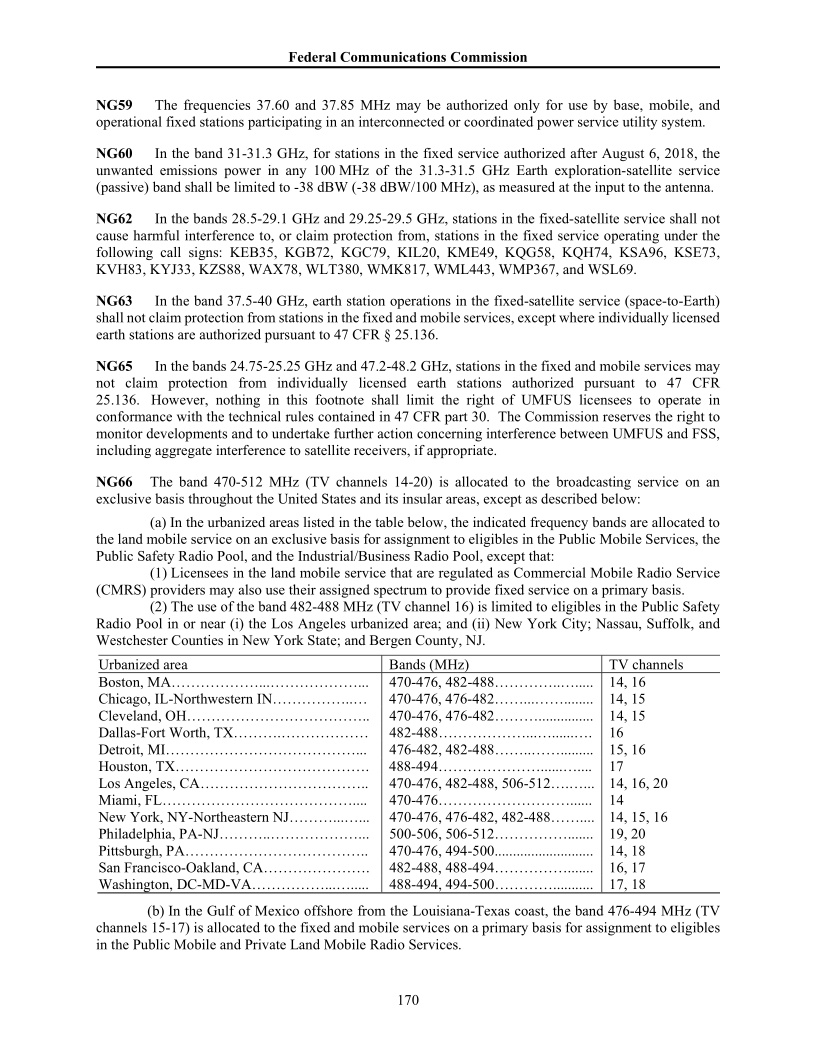
\includegraphics[width=0.8\textwidth]{test-resultaten/6/original.jpg}
    \caption{Origineel document.}
\end{figure}

\begin{figure}[H]
    \centering
    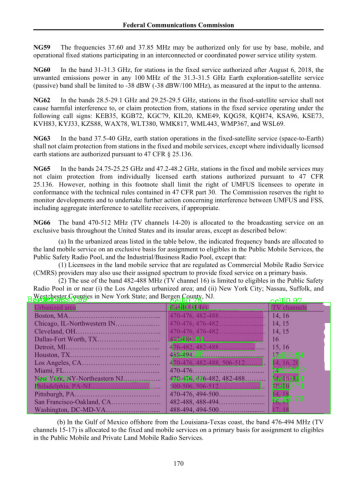
\includegraphics[width=0.8\textwidth]{test-resultaten/6/detected_tables.png}
    \caption{Gedetecteerde tabellen.}
\end{figure}

Getransformeerde tabellen met algoritme A:

\begin{tabular}{lll}
\toprule
{} &                                    ‘Urbanized area &                                        TV channels \\
\midrule
0 &  Dallas-Fort Worth, TX.\textbackslash n\textbackslash nDetroit, MI\textbackslash n\textbackslash nHoust... &  16\textbackslash n\textbackslash n15, 16\textbackslash n7\textbackslash n\textbackslash n14, 16.\textbackslash n14\textbackslash n\textbackslash n14,15\textbackslash n19, 2... \\
\bottomrule
\end{tabular}

Getransformeerde tabellen met algoritme B:

\begin{tabular}{llll}
\toprule
{} &                                 Urbanized area &                         Bands (MH) &   TV channels \\
\midrule
0  &                                  Boston, MA... &                  AT0-AT6, 482-488, &         14,16 \\
1  &                   Chicago, 1L-Northwestern IN. &                   410-476, 476-482 &          141s \\
2  &                               Cleveland, OH... &                470-476, 476-482... &        14,15, \\
3  &                         Dallas-Fort Worth, TX. &                           482-488, &            16 \\
4  &                                    Detroit, MI &                  476-482, 482-488. &         15,16 \\
5  &                                   Houston, TX. &                           488-494, &            17 \\
6  &                               Los Angeles, CA. &         470-476, 482-488, 506-512. &    14, 16, 20 \\
7  &  Miami. EL...... New York, NY-1 Northeastem NI &  AT0AT6, AT0AT6, 476-482, 482-488. &  14 14, 15,16 \\
8  &                           Philadelphia, PA-NJ. &                  500-506, 506-512. &        19, 20 \\
9  &                                Pittsburgh, PA. &                  470-476, 494-500, &         14.18 \\
10 &                      San Francisco-Oakland, €. &                  482-488, 488-494. &        16,17, \\
11 &                          Washington, DC-MD-VA. &                  488-494, 494-500. &        17,18, \\
\bottomrule
\end{tabular}
\section{Document 7}

\begin{figure}[H]
    \centering
    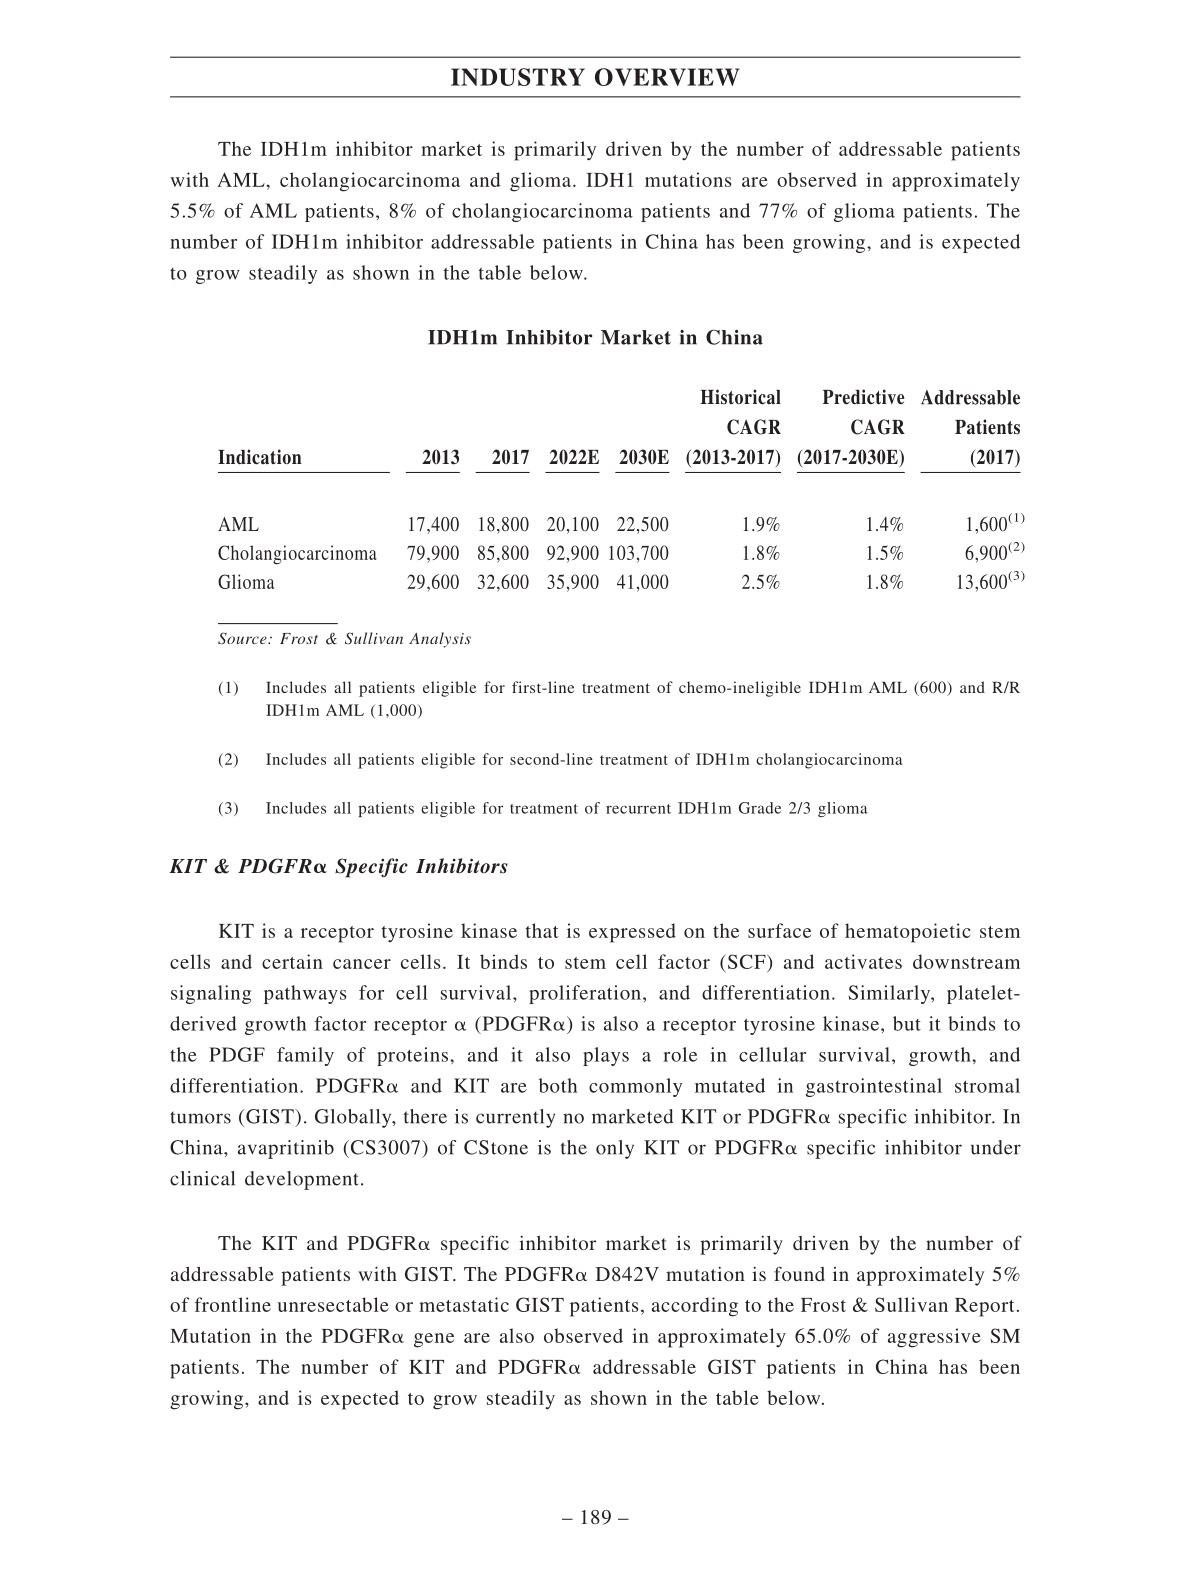
\includegraphics[width=0.8\textwidth]{test-resultaten/7/original.jpg}
    \caption{Origineel document.}
\end{figure}

\begin{figure}[H]
    \centering
    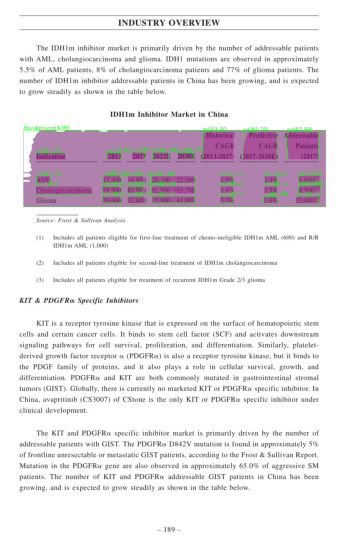
\includegraphics[width=0.8\textwidth]{test-resultaten/7/detected_tables.png}
    \caption{Gedetecteerde tabellen.}
\end{figure}

Getransformeerde tabellen met algoritme A:

\begin{tabular}{lllllllll}
\toprule
{} &          Indication &    2013 &    2017 &           2022E &   2030E & Historical\textbackslash nCAGR\textbackslash n(2013-2017) & Predictive\textbackslash nCAGE\textbackslash n2017-2030E & ddressable\textbackslash nPatients\textbackslash n(2017) \\
\midrule
0 &                 AML &  17.400 &  18.800 &   20.100 22.500 &  22,500 &                          1.9\% &                         1.4\% &                        1,600 \\
1 &  Cholangiocarcinoma &  79.900 &  85.800 &  92.900 103.700 &    1.8\% &                          1.5\% &                      6,900?) &                         None \\
2 &              Glioma &  29.600 &  32.600 &    35 000 ALONO &  41,000 &                           25\% &                         1.8\% &                       13,600 \\
\bottomrule
\end{tabular}

Getransformeerde tabellen met algoritme B:

\begin{tabular}{lllllllll}
\toprule
{} &   Historical &    Predictive & Addressable &                 NaN &     NaN &     NaN &     NaN &      NaN \\
\midrule
0 &         CAGR &          CAGR &    Patients &                None &    None &    None &    None &     None \\
1 &  (2013-2017) &  (2017-2030E) &      (2017) &          Indication &    2013 &    2017 &    None &     None \\
2 &         1.9\% &          1.4\% &       1,600 &                 AML &  17,400 &  18,800 &  20,100 &   22,500 \\
3 &         1.8\% &          1.5\% &       6,900 &  Cholangiocarcinoma &  79,900 &  85,800 &  92,900 &  103,700 \\
4 &         2.5\% &          1.8\% &      13,600 &              Glioma &  29,600 &  32,600 &  35,900 &   41,000 \\
\bottomrule
\end{tabular}
\section{Document 8}

\begin{figure}[H]
    \centering
    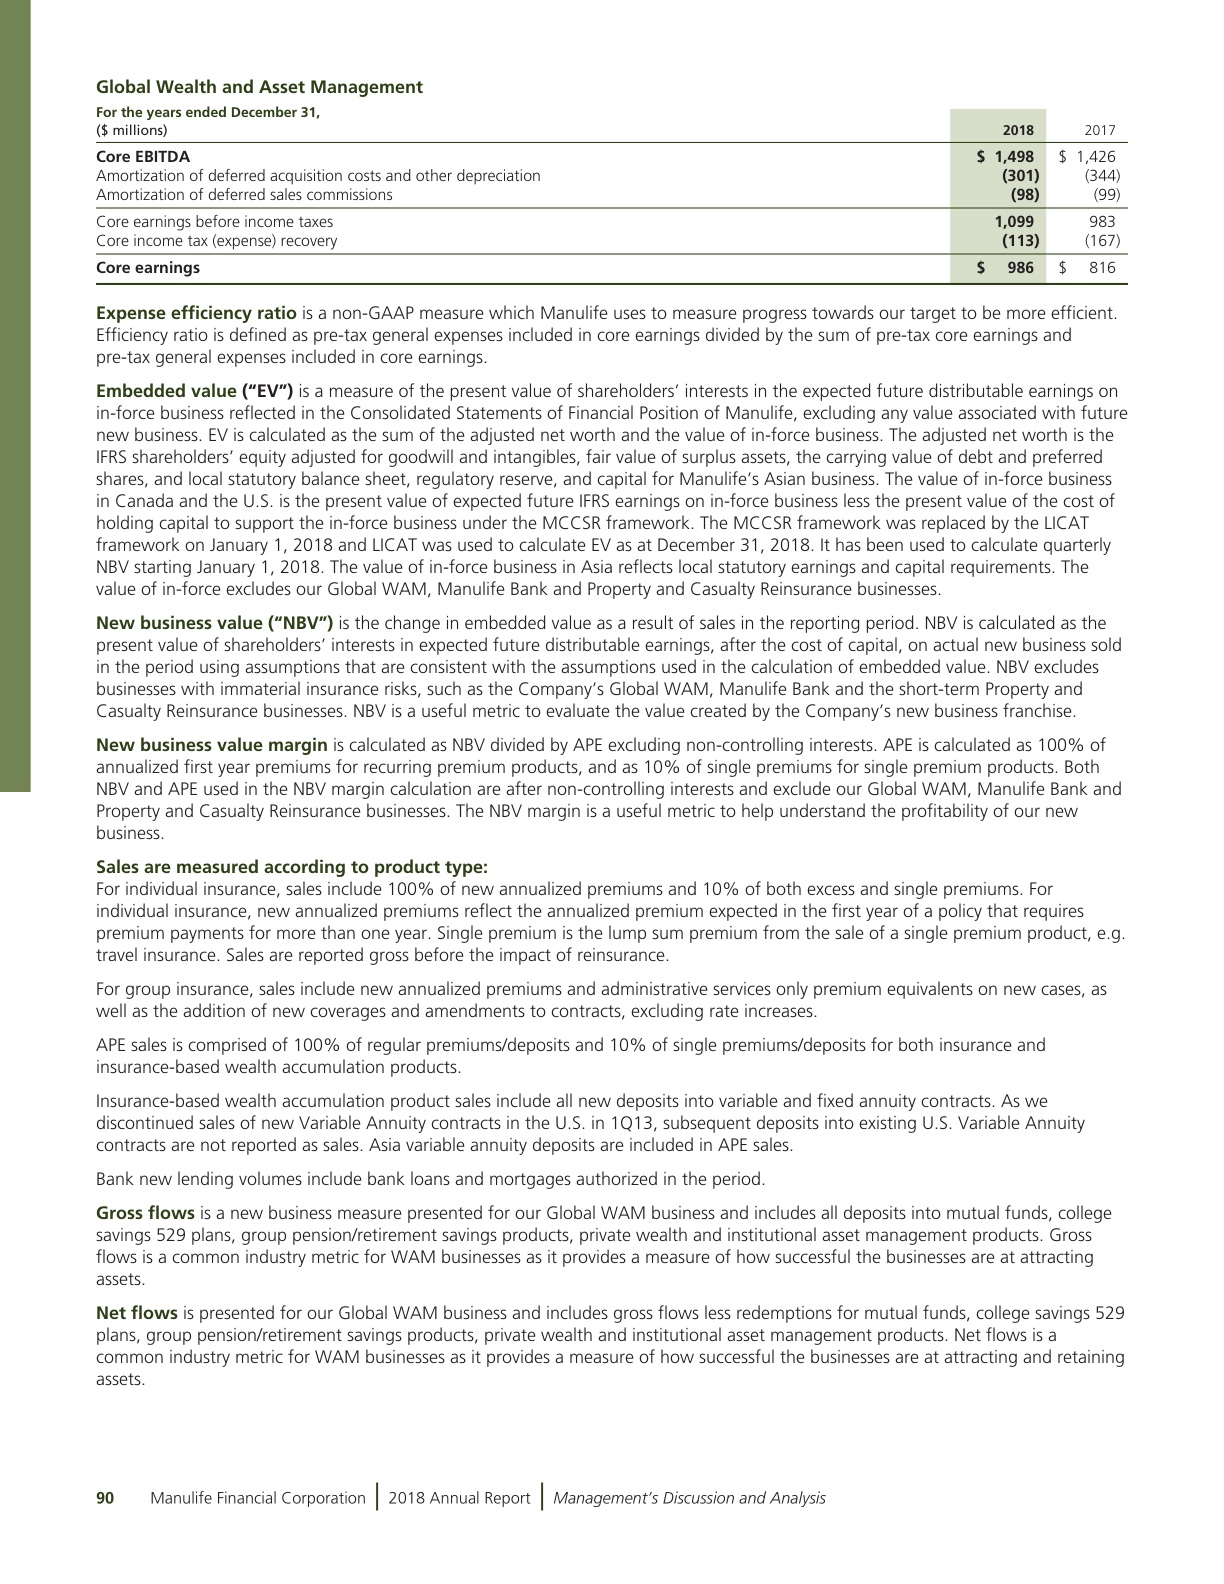
\includegraphics[width=0.8\textwidth]{test-resultaten/8/original.jpg}
    \caption{Origineel document.}
\end{figure}

\begin{figure}[H]
    \centering
    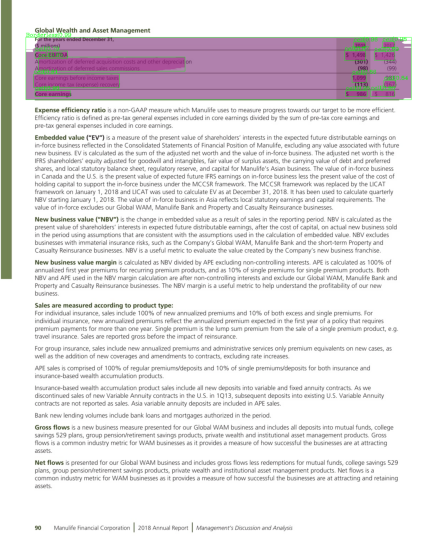
\includegraphics[width=0.8\textwidth]{test-resultaten/8/detected_tables.png}
    \caption{Gedetecteerde tabellen.}
\end{figure}

Getransformeerde tabellen met algoritme A:

\begin{tabular}{llll}
\toprule
{} &     For the years ended December 31,\textbackslash n(\$ millions) &          2018 &        2017 \\
\midrule
0 &  mortization of deferred acquisition costs and ... &       \$ 1,498 &     \$ 1,426 \\
1 &  Core earnings before income taxes\textbackslash nCore income... &  1,099\textbackslash n(113) &  983\textbackslash n(167) \\
2 &                                      Core earnings &        S\$ 986 &       \$ 816 \\
\bottomrule
\end{tabular}

Getransformeerde tabellen met algoritme B:

\begin{tabular}{lllll}
\toprule
{} &                   For the years ended December 31, &     NaN &           NaN &      NaN \\
\midrule
0 &                                       (§ millions) &    2018 &          None &     2017 \\
1 &                                        Core EBITDA &  \$1,498 &          None &  \$ 1,426 \\
2 &  Amortization of deferred acquisition costs and... &   (301) &  depreciation &    (344) \\
3 &         Amortization of deferred sales commissions &    (9a) &          None &     (99) \\
4 &                  Core earnings before income taxes &   1,099 &          None &      983 \\
5 &                        Core tax (expense) recovery &   (113) &          None &    (167) \\
6 &                                      Core earnings &   \$ 986 &          None &    \$ 816 \\
\bottomrule
\end{tabular}
\section{Document 9}

\begin{figure}[H]
    \centering
    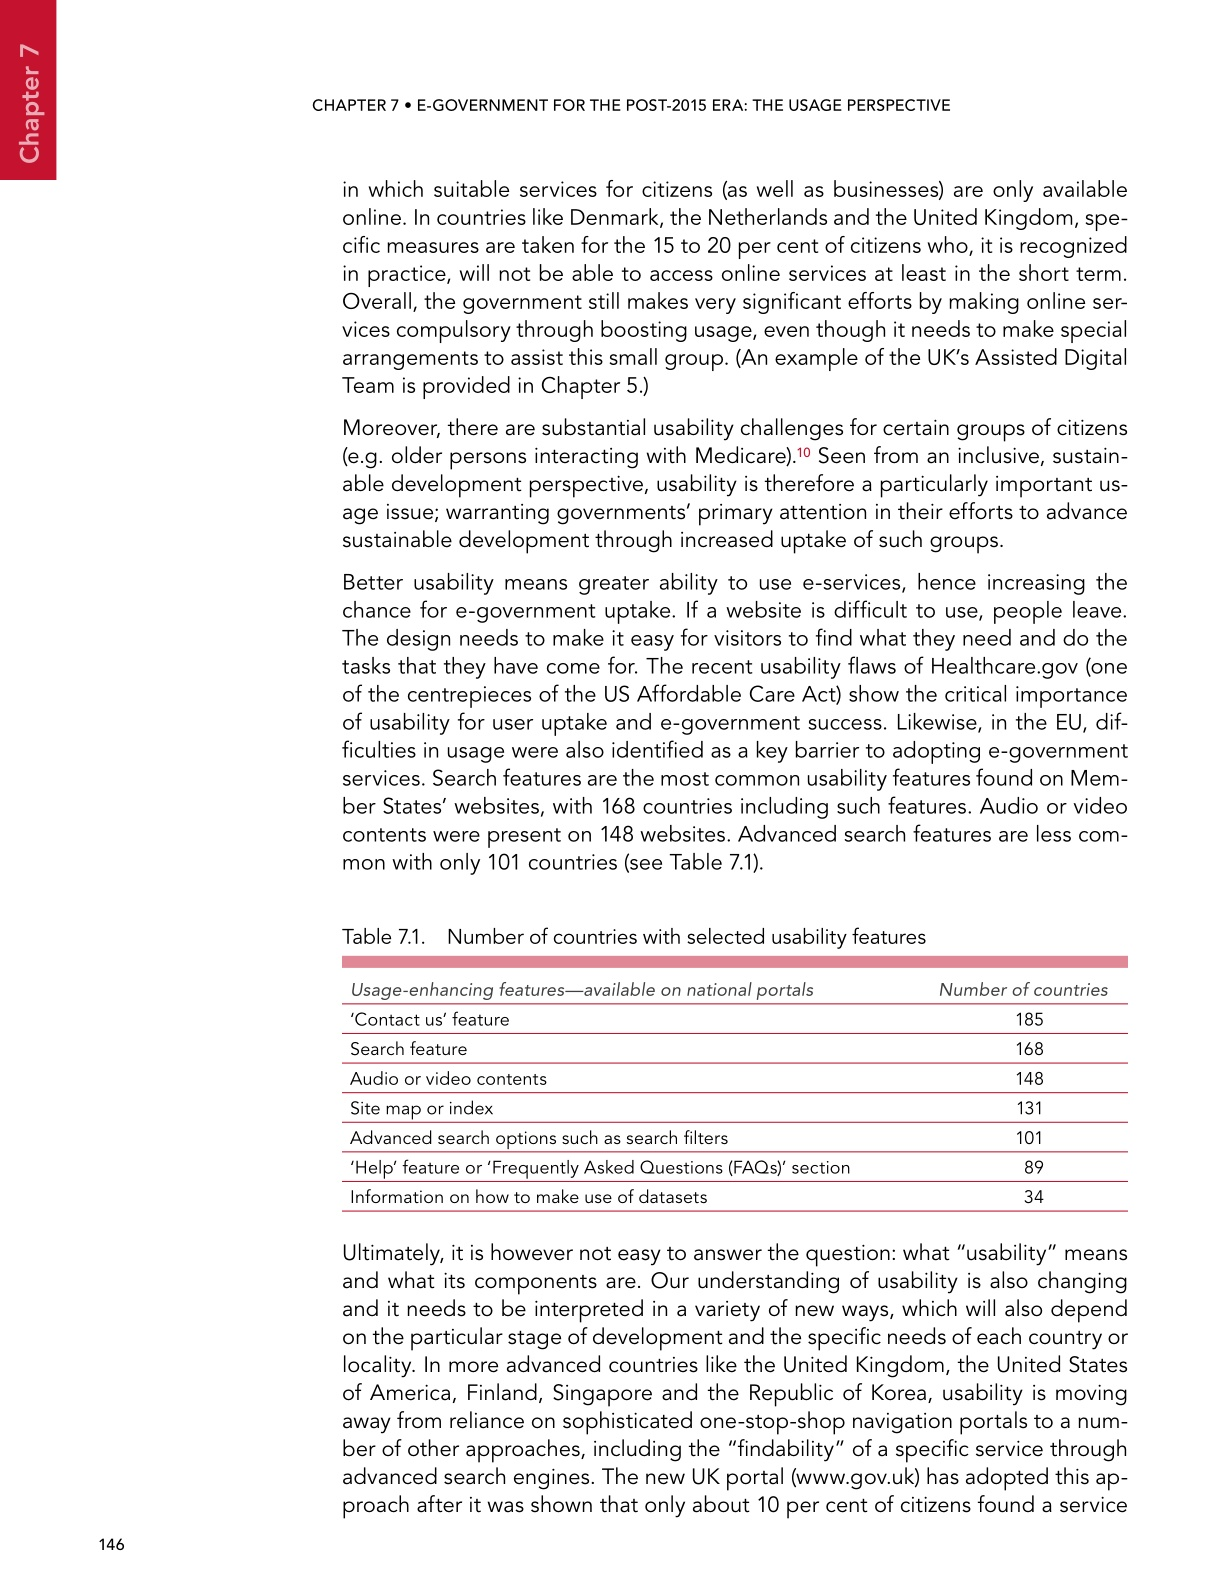
\includegraphics[width=0.8\textwidth]{test-resultaten/9/original.jpg}
    \caption{Origineel document.}
\end{figure}

\begin{figure}[H]
    \centering
    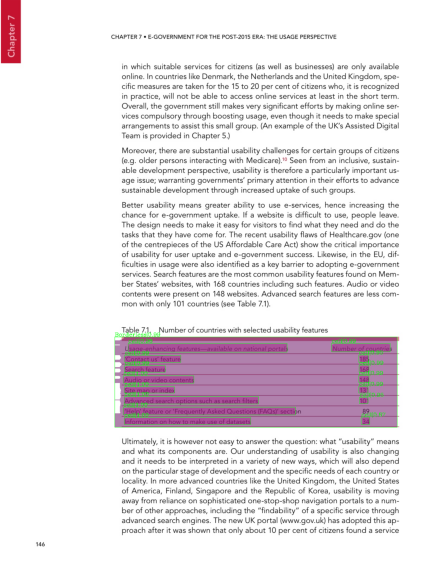
\includegraphics[width=0.8\textwidth]{test-resultaten/9/detected_tables.png}
    \caption{Gedetecteerde tabellen.}
\end{figure}

Getransformeerde tabellen met algoritme A:

\begin{tabular}{lll}
\toprule
{} & Usage-enhancing features—available on national portals & Number of countries \\
\midrule
0 &                               ‘Contact us’ feature &                 185 \\
1 &                                     Search feature &                 168 \\
2 &                            Audio or video contents &                 148 \\
3 &                                  Site map or index &                 131 \\
4 &     Advanced search options such as search filters &                 101 \\
5 &  ‘Help’ feature or ‘Frequently Asked Questions ... &                 B89 \\
6 &         Information on how to make use of datasets &                  34 \\
\bottomrule
\end{tabular}

Getransformeerde tabellen met algoritme B:

\begin{tabular}{lll}
\toprule
{} & Usage-enhancing features—available on national portals & Number of countries \\
\midrule
0 &                               ‘Contact us’ feature &                 185 \\
1 &                                     Search feature &                 168 \\
2 &                            Audio or video contents &                 148 \\
3 &                                  Site map or index &                 131 \\
4 &     Advanced search options such as search filters &                 101 \\
5 &  ‘Help’ feature or ‘Frequently Asked Questions ... &                  89 \\
6 &         Information on how to make use of datasets &                  34 \\
\bottomrule
\end{tabular}
\section{Document 10}

\begin{figure}[H]
    \centering
    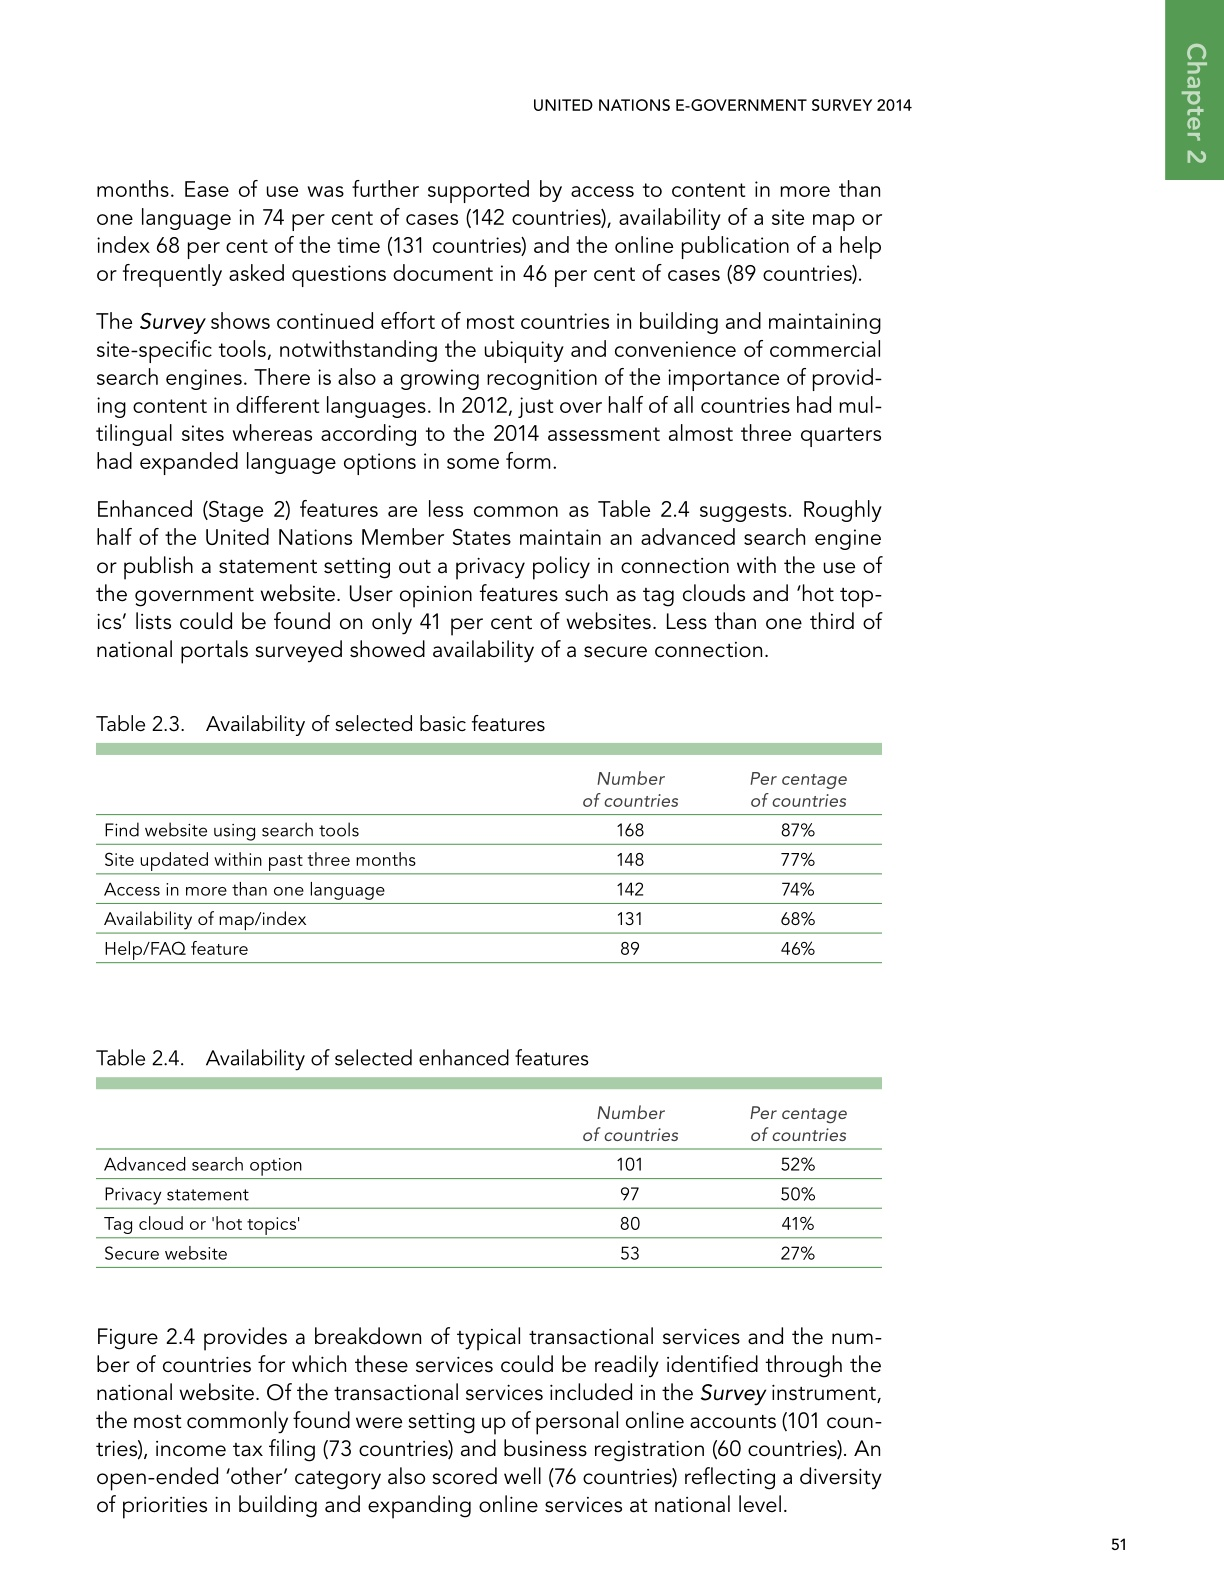
\includegraphics[width=0.8\textwidth]{test-resultaten/10/original.jpg}
    \caption{Origineel document.}
\end{figure}

\begin{figure}[H]
    \centering
    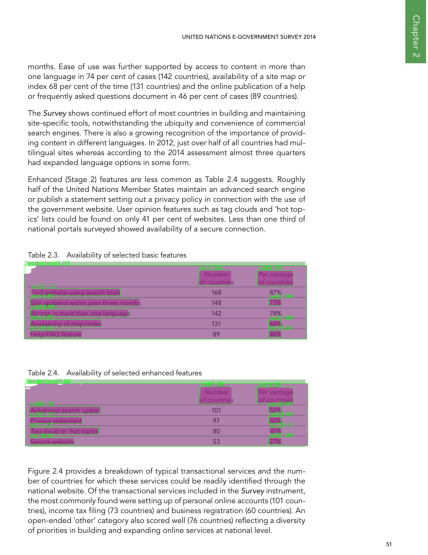
\includegraphics[width=0.8\textwidth]{test-resultaten/10/detected_tables.png}
    \caption{Gedetecteerde tabellen.}
\end{figure}

Getransformeerde tabellen met algoritme A:

\begin{tabular}{lll}
\toprule
{} &      Number\textbackslash nof countries & Per centage\textbackslash nof countries \\
\midrule
0 &    Advanced search optior &                       52\% \\
1 &         Privacy statement &                       50\% \\
2 &  Taq cloud or ‘hot topics &                       AIM \\
3 &            Secure website &                       27\% \\
\bottomrule
\end{tabular}

\begin{tabular}{lll}
\toprule
{} &                   Number\textbackslash nof countries & Per centage\textbackslash nof countries \\
\midrule
0 &        Find website using search tools &                       87\% \\
1 &  Site updated within past three months &                       77\% \\
2 &       Access in more than one lanquaas &                       TA\% \\
3 &              Availability of map/inde> &                       68\% \\
4 &                       Help/FAQ feature &                       Ab\% \\
\bottomrule
\end{tabular}

Getransformeerde tabellen met algoritme B:

\begin{tabular}{llll}
\toprule
{} &        Number &   Per centage &                        NaN \\
\midrule
0 &  of countries &  of countries &                       None \\
1 &           101 &           52\% &     Advanced search option \\
2 &            97 &           50\% &          Privacy statement \\
3 &            80 &           41\% &  Tag cloud or ‘hot topics’ \\
4 &            53 &           27\% &             Secure website \\
\bottomrule
\end{tabular}

\begin{tabular}{llll}
\toprule
{} &        Number &   Per centage &                                    NaN \\
\midrule
0 &  of countries &  of countries &                                   None \\
1 &           168 &           87\% &        Find website using search tools \\
2 &           148 &           71\% &  Site updated within past three months \\
3 &           142 &           74\% &       Access in more than one language \\
4 &           131 &           68\% &              Availability of map/index \\
5 &            89 &           46\% &                       Help/FAQ feature \\
\bottomrule
\end{tabular}
\section{Document 11}

\begin{figure}[H]
    \centering
    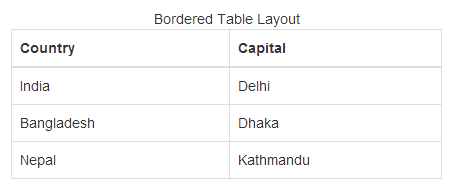
\includegraphics[width=0.8\textwidth]{test-resultaten/11/original.png}
    \caption{Origineel document.}
\end{figure}

\begin{figure}[H]
    \centering
    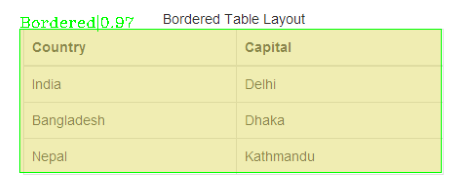
\includegraphics[width=0.8\textwidth]{test-resultaten/11/detected_tables.png}
    \caption{Gedetecteerde tabellen.}
\end{figure}

Getransformeerde tabellen met algoritme A:

\begin{tabular}{lll}
\toprule
{} &     Country &    Capital \\
\midrule
0 &       India &      Delhi \\
1 &  Bangladesh &      Dhaka \\
2 &       Nepal &  Kathmandu \\
\bottomrule
\end{tabular}

Getransformeerde tabellen met algoritme B:

\begin{tabular}{lll}
\toprule
{} &     Country &    Capital \\
\midrule
0 &       India &      Delhi \\
1 &  Bangladesh &      Dhaka \\
2 &       Nepal &  Kathmandu \\
\bottomrule
\end{tabular}
\section{Document 12}

\begin{figure}[H]
    \centering
    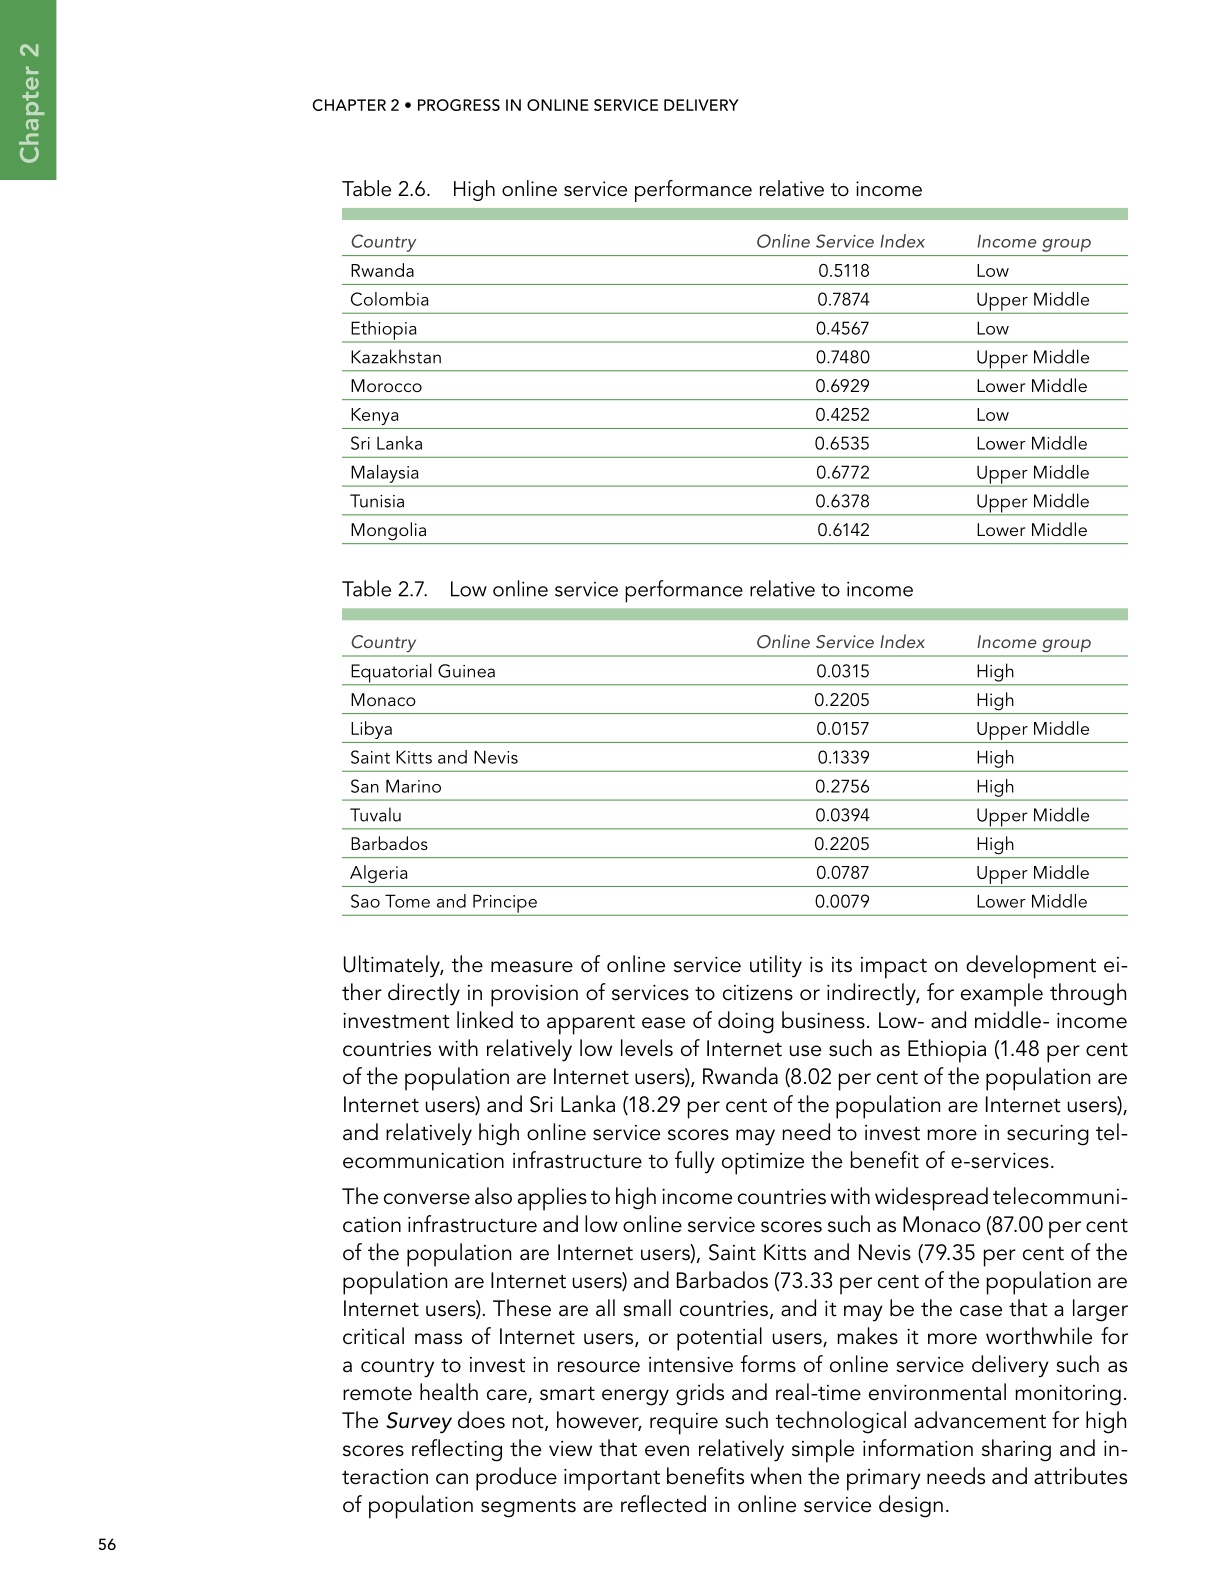
\includegraphics[width=0.8\textwidth]{test-resultaten/12/original.png}
    \caption{Origineel document.}
\end{figure}

\begin{figure}[H]
    \centering
    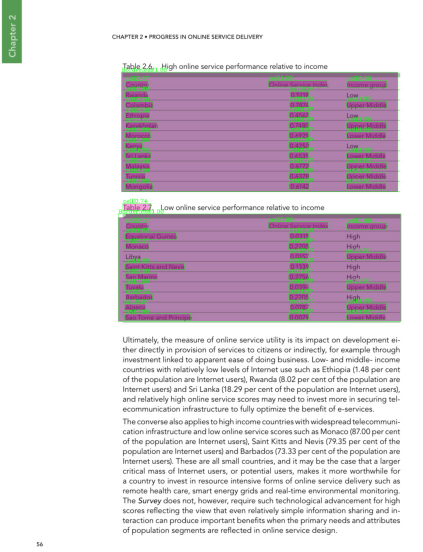
\includegraphics[width=0.8\textwidth]{test-resultaten/12/detected_tables.png}
    \caption{Gedetecteerde tabellen.}
\end{figure}

Getransformeerde tabellen met algoritme A:

Getransformeerde tabellen met algoritme B:
\section{Document 13}

\begin{figure}[H]
    \centering
    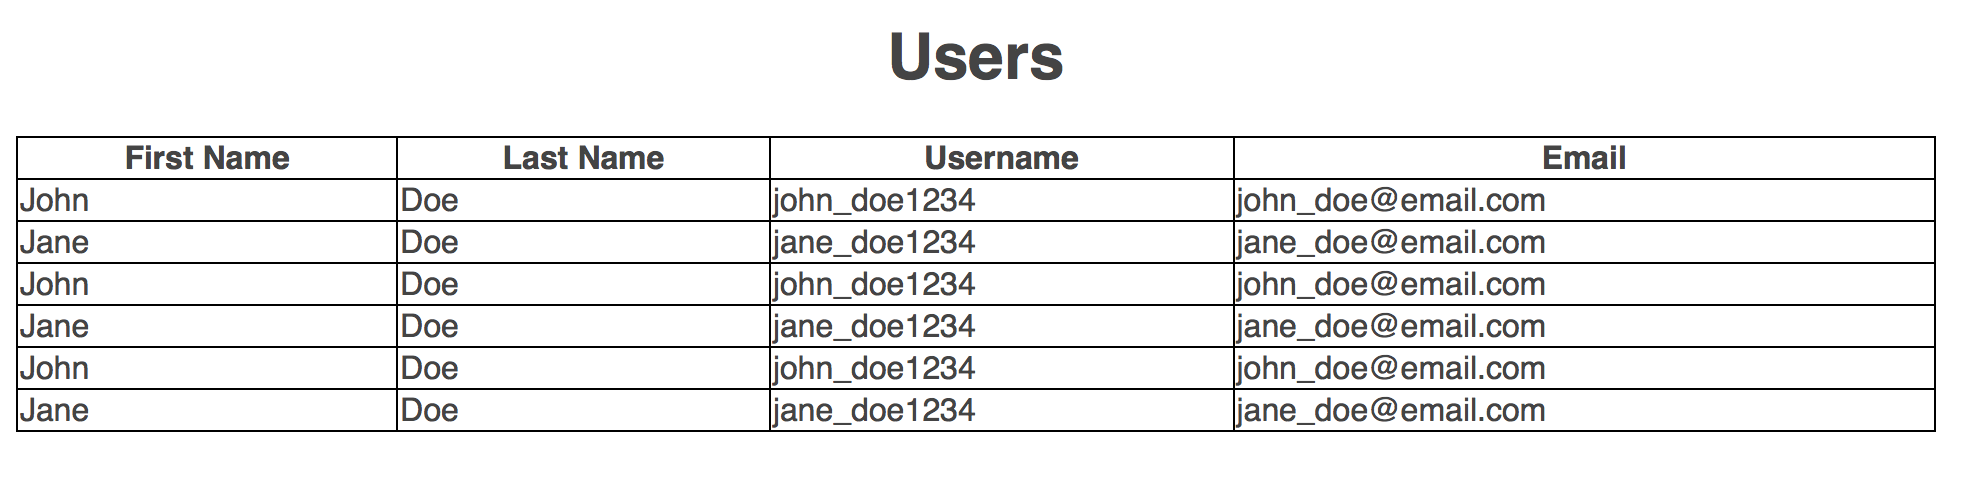
\includegraphics[width=0.8\textwidth]{test-resultaten/13/original.png}
    \caption{Origineel document.}
\end{figure}

\begin{figure}[H]
    \centering
    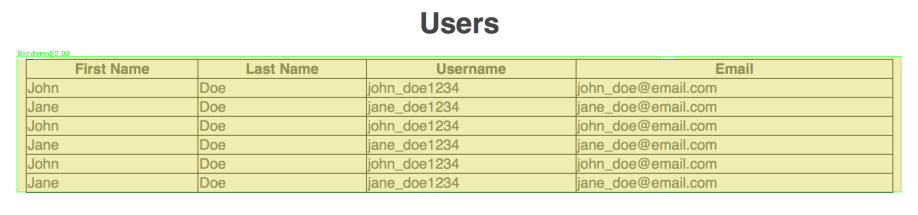
\includegraphics[width=0.8\textwidth]{test-resultaten/13/detected_tables.png}
    \caption{Gedetecteerde tabellen.}
\end{figure}

Getransformeerde tabellen met algoritme A:

Getransformeerde tabellen met algoritme B:
\section{Document 14}

\begin{figure}[H]
    \centering
    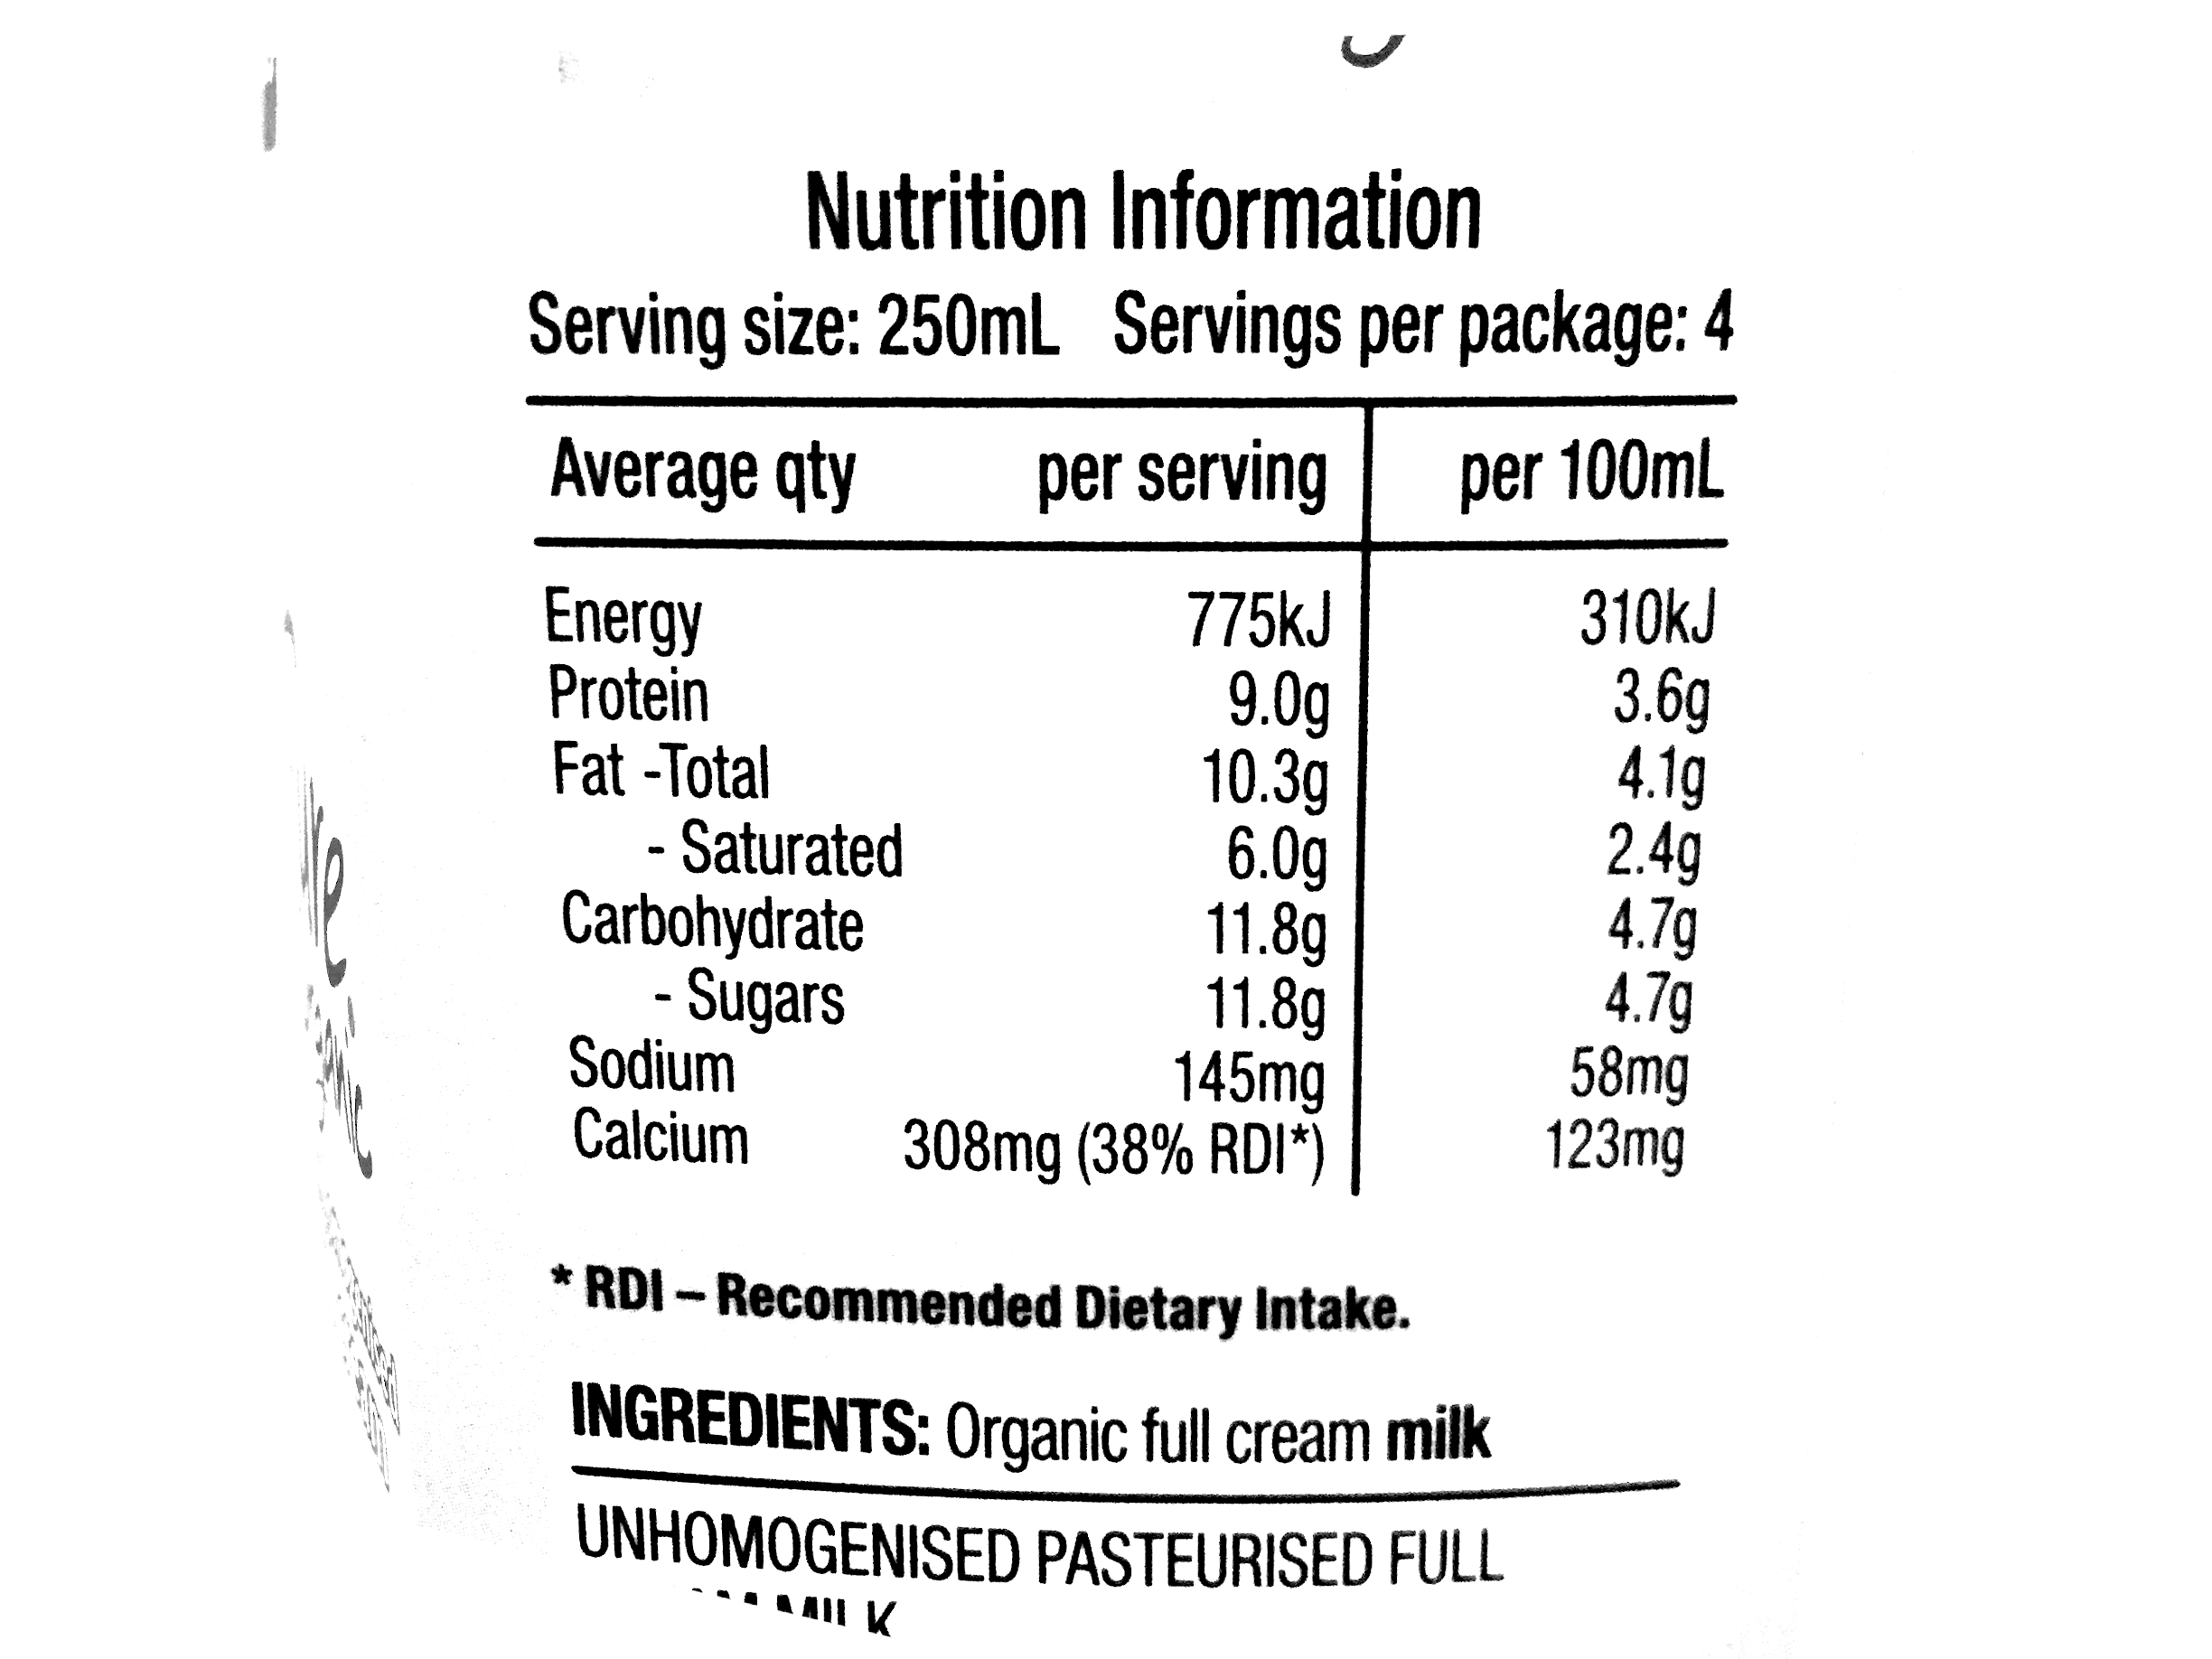
\includegraphics[width=0.8\textwidth]{test-resultaten/14/original_b/original.png}
    \caption{Origineel document.}
\end{figure}

\begin{figure}[H]
    \centering
    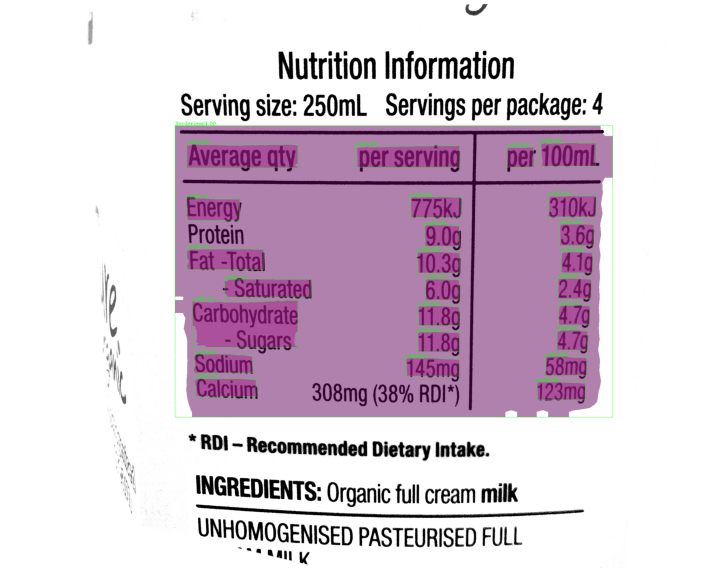
\includegraphics[width=0.8\textwidth]{test-resultaten/14/original_b/detected_tables.png}
    \caption{Gedetecteerde tabellen.}
\end{figure}

Getransformeerde tabellen met algoritme A:

Tabeltransformatie gefaald.

Getransformeerde tabellen met algoritme B:

\begin{tabular}{llllll}
\toprule
{} &   Average aty &   per & serving &    NaN &  100mL \\
\midrule
0 &        Energy &  None &   775kd &   None &  310kJ \\
1 &       Protein &  None &    9.09 &   None &   3.69 \\
2 &    Fat -Total &  None &   10.3g &   None &    41g \\
3 &   - Saturated &  None &    6.0g &   None &   2.49 \\
4 &  Carbohydrate &  None &   11.89 &   None &    4/9 \\
5 &      - Sugars &  None &   11.89 &   None &    479 \\
6 &        sodium &  None &    None &   None &   None \\
7 &          None &  None &   145mg &   None &   58mg \\
8 &       Calcium &  (38\% &   RDI*) &  308mg &  123mg \\
\bottomrule
\end{tabular}
\section{Document 15}

\begin{figure}[H]
    \centering
    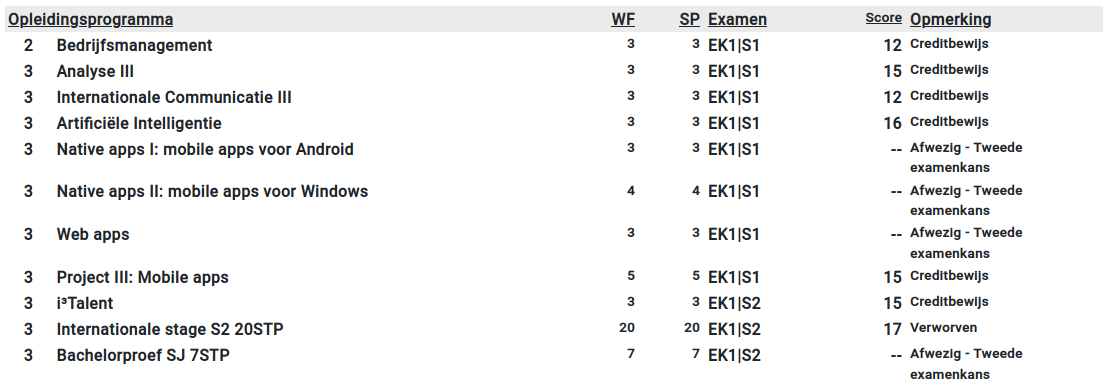
\includegraphics[width=0.8\textwidth]{test-resultaten/15/orignal.png}
    \caption{Origineel document.}
\end{figure}

\begin{figure}[H]
    \centering
    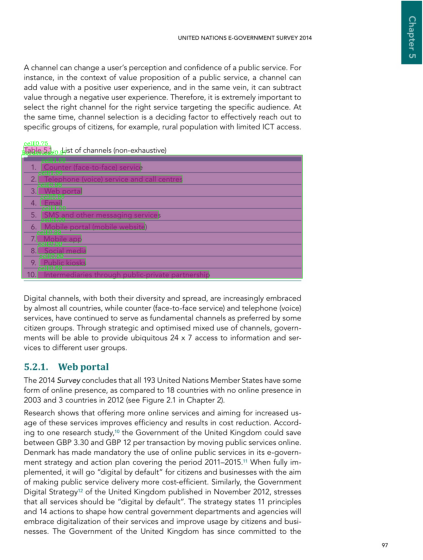
\includegraphics[width=0.8\textwidth]{test-resultaten/1/detected_tables.png}
    \caption{Gedetecteerde tabellen.}
\end{figure}

Getransformeerde tabellen met algoritme A:

\begin{tabular}{llll}
\toprule
{} &                                Opleidingsprogramma &         WE & 12 Creditbewi\textbackslash n15 Creditbewljs\textbackslash n12 Creditbewijs\textbackslash n16 Creditbewijs \\
\midrule
0 &               2 Bedrijfsmanagement\textbackslash n3. Analyse Ill &   3 EK1/S1 &                   12 Creditbewijs\textbackslash n15 Creditbewijs \\
1 &  3 Internationale Communicatie III\textbackslash n3. Artifici... &   3 EK1/S1 &                   12 Creditbewijs\textbackslash n16 Creditbewijs \\
2 &            Native apps |: mobile apps voor Android &   3 EK1/S1 &                                   Afwezig - Tweede \\
3 &      3 .\textasciitilde =Native apps II: mobile apps voor Windows &   4 EK1/S1 &                                   Afwezig - Tweede \\
4 &                                           Web apps &   3 FK1IS1 &                                   Afwezig - Tweede \\
5 &                     3 \textasciitilde \textasciitilde  \textasciitilde Project Ill: Mobile apps &   5 EK1/S1 &                                    15 Creditbewijs \\
6 &                                             Talent &   3 EK1IS2 &                                    15 Creditbewijs \\
7 &  Internationale stage S2 20STP\textbackslash nBachelorproef S... &  20 EK1/S2 &                                               None \\
8 &                          3  =Bachelorproef SJ 7STP &   7 EK1IS2 &                      Afwezig - Tweede\textbackslash n‘examenkans \\
\bottomrule
\end{tabular}

Getransformeerde tabellen met algoritme B:

\begin{tabular}{llll}
\toprule
{} &                          Opleidingsprogramma &    ‘SP Examen &  Seore Opmerking \\
\midrule
0  &                         2 Bedrijfsmanagement &      3 EK1|S1 &      Creditbewjs \\
1  &                                3 Analyse Ill &      3 EK1|S1 &      Creditbewjs \\
2  &            3 Internationale Communicatie Ill &      3 EK1|S1 &      Creditbewjs \\
3  &                  3 Artificiéle Intelligentie &      3 EK1|S1 &      Creditbewjs \\
4  &   3. Native apps |: mobile apps voor Android &      3 EK1|S1 &  Afwezig- Tweede \\
5  &  3. Native apps Il: mobile apps voor Windows &      4 EK1|S1 &  Afwezig- Tweede \\
6  &                                  3. Web apps &      3 EK1|S1 &  Afwezig- Tweede \\
7  &                   3 Project Ill: Mobile apps &      \$ EK1|S1 &   15 Creditbewjs \\
8  &                                    3 iTalent &      3 EK1|S2 &   15 Creditbewjs \\
9  &              3 Internationale stage \$2 20STP &  20 20 EK1|S2 &      7 Verworven \\
10 &                      3 Bachelorproef SJ 7STP &           7 7 &  Afwezig- Tweede \\
11 &                                         None &          None &       examenkans \\
12 &                                         None &          None &       examenkans \\
13 &                                         None &          None &       examenkans \\
\bottomrule
\end{tabular}
\section{Document 16}

\begin{figure}[H]
    \centering
    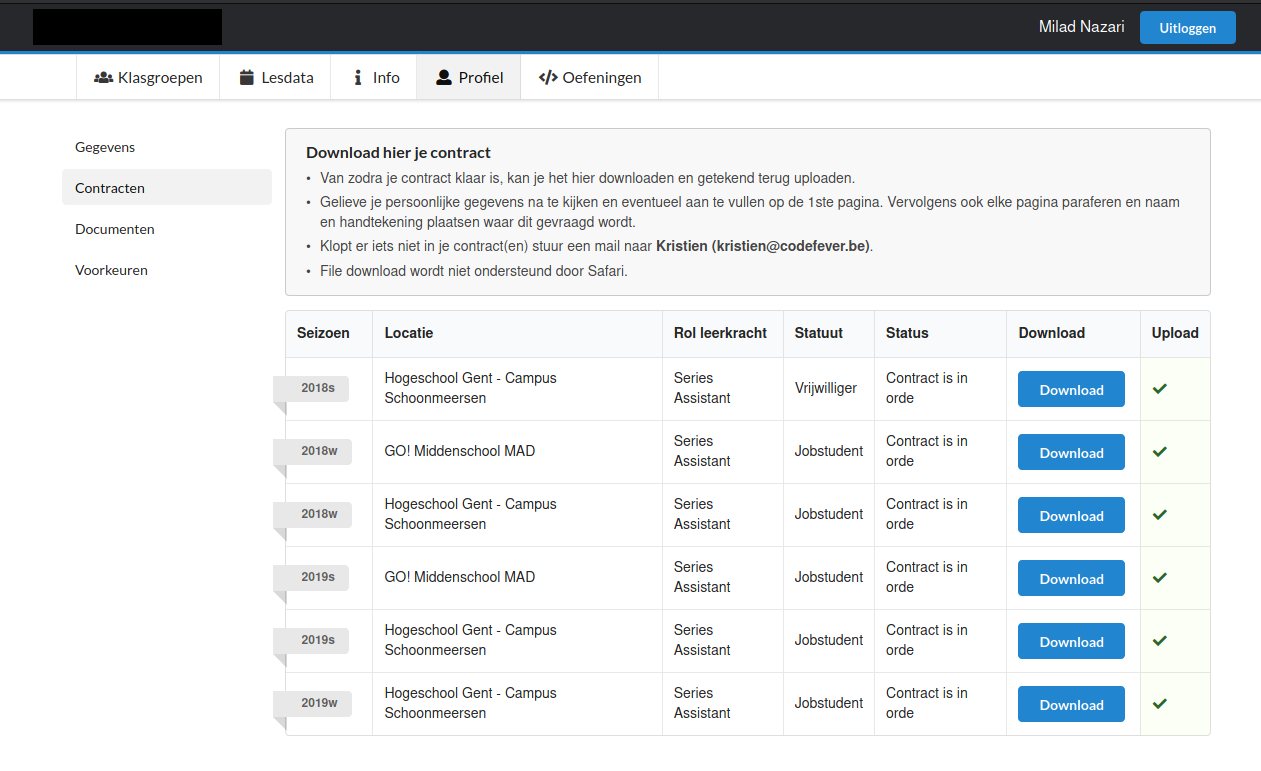
\includegraphics[width=0.8\textwidth]{test-resultaten/16/original.png}
    \caption{Origineel document.}
\end{figure}

\begin{figure}[H]
    \centering
    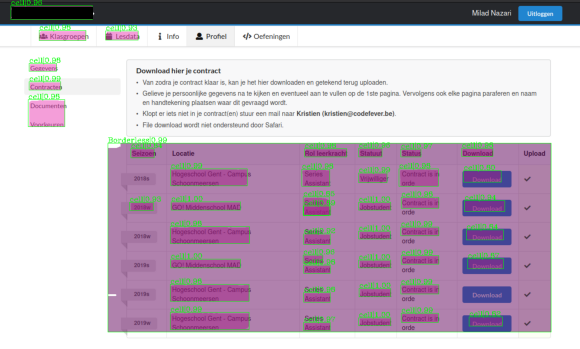
\includegraphics[width=0.8\textwidth]{test-resultaten/16/detected_tables.png}
    \caption{Gedetecteerde tabellen.}
\end{figure}

Getransformeerde tabellen met algoritme A:

\begin{tabular}{lllllll}
\toprule
{} & Seizoen &                                  Locatie &     Rol leerkrachi &       Statuut &                 Status &  Download \\
\midrule
0 &   2018s &  Hogeschool Gent - Campus\textbackslash nSchoonmeersen &  Series\textbackslash nAssistant &  Vrijwilliger &  Contract is in\textbackslash ncorde &        as \\
1 &   2018w &                     GO! Middenschool MAD &  Series\textbackslash nAssistant &    Jobstudent &  Contract is in\textbackslash ncorde &  Download \\
2 &   2018w &  Hogeschool Gent - Campus\textbackslash nSchoonmeersen &  Series\textbackslash nAssistant &    Jobstudent &  Contract is in\textbackslash ncorde &        as \\
3 &   2019s &                     GO! Middenschool MAD &  Series\textbackslash nAssistant &    Jobstudent &  Contract is in\textbackslash ncorde &  Download \\
4 &   2019s &  Hogeschool Gent - Campus\textbackslash nSchoonmeersen &  Series\textbackslash nAssistant &    Jobstudent &  Contract is in\textbackslash ncorde &        as \\
5 &   2019W &  Hogeschool Gent - Campus\textbackslash nSchoonmeersen &  Series\textbackslash nAssistant &    Jobstudent &  Contract is in\textbackslash ncorde &        as \\
\bottomrule
\end{tabular}


Getransformeerde tabellen met algoritme B:

\begin{tabular}{lllllll}
\toprule
{} & Seizoen &                                 Locatie &    Rol leerkracht &       Statuut &                Status &  Download \\
\midrule
0 &   20188 &  Hogeschool Gent - Campus Schoonmeersen &  Series Assistant &  Vrijwilliger &  Contract is in corde &  Download \\
1 &   20180 &                    GO! Middenschool MAD &  Series Assistant &    dobstudent &  Contract is in corde &  Download \\
2 &   20180 &  Hogeschool Gent - Campus Schoonmeersen &  Series Assistant &    dobstudent &  Contract is in corde &  Download \\
3 &   20198 &                    GO! Middenschool MAD &  Series Assistant &    dobstudent &  Contract is in corde &  Download \\
4 &   20198 &  Hogeschool Gent - Campus Schoonmeersen &  Series Assistant &    dobstudent &  Contract is in corde &  Download \\
5 &   2019" &  Hogeschool Gent - Campus Schoonmeersen &  Series Assistant &    dobstudent &   Contract is in orde &  Download \\
\bottomrule
\end{tabular}
\section{Document 17}

\begin{figure}[H]
    \centering
    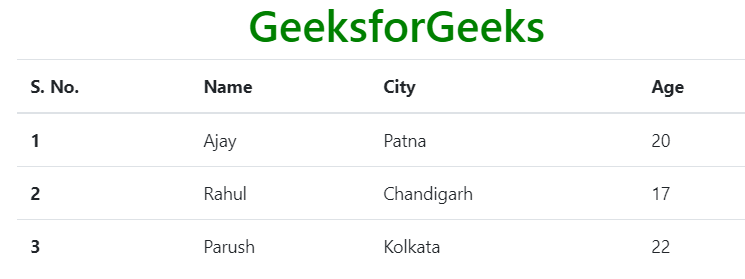
\includegraphics[width=0.8\textwidth]{test-resultaten/17/original.png}
    \caption{Origineel document.}
\end{figure}

\begin{figure}[H]
    \centering
    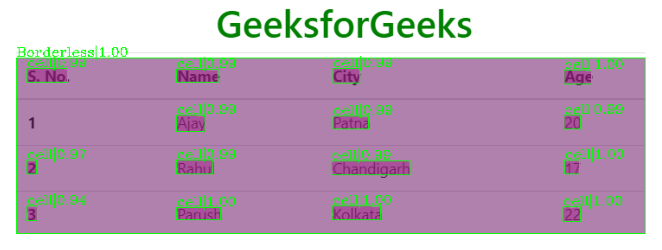
\includegraphics[width=0.8\textwidth]{test-resultaten/17/detected_tables.png}
    \caption{Gedetecteerde tabellen.}
\end{figure}

Getransformeerde tabellen met algoritme A:

\begin{tabular}{lllll}
\toprule
{} & S. No. &    Name &        City & Age \\
\midrule
0 &      1 &    Ajay &       Patna &  20 \\
1 &      2 &   Rahul &  Chandigarh &  17 \\
2 &      3 &  Parush &     Kolkata &  22 \\
\bottomrule
\end{tabular}

Getransformeerde tabellen met algoritme B:

\begin{tabular}{lllll}
\toprule
{} & S.No. &    Name &        City & Age \\
\midrule
0 &     1 &    Ajay &       Patna &  20 \\
1 &     2 &   Rahul &  Chandigarh &   7 \\
2 &     3 &  Parush &     Kolkata &  22 \\
\bottomrule
\end{tabular}
\section{Document 18}

\begin{figure}[H]
    \centering
    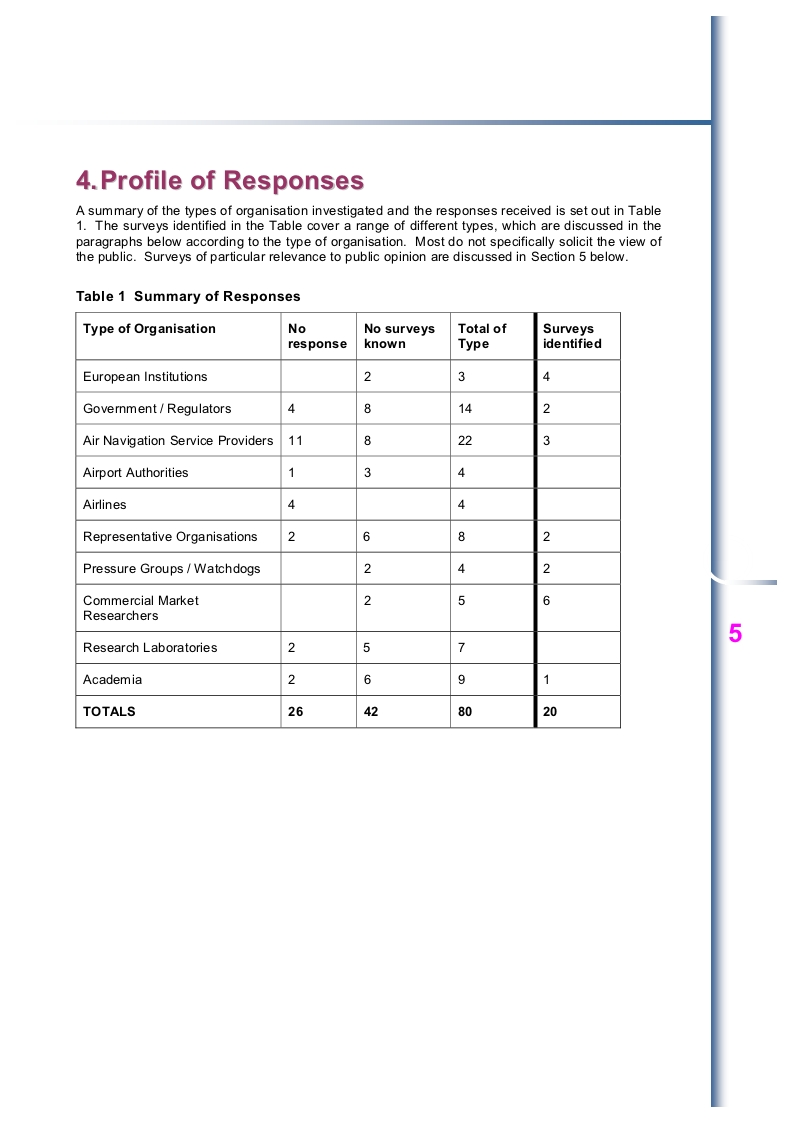
\includegraphics[width=0.8\textwidth]{test-resultaten/18/original.png}
    \caption{Origineel document.}
\end{figure}

\begin{figure}[H]
    \centering
    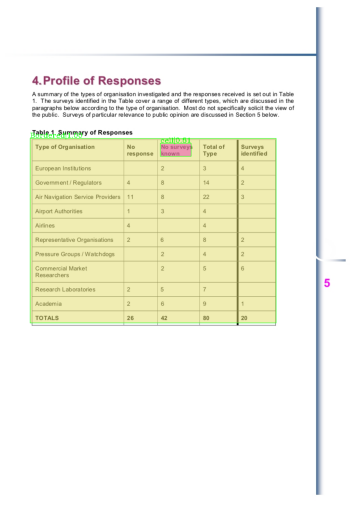
\includegraphics[width=0.8\textwidth]{test-resultaten/18/detected_tables.png}
    \caption{Gedetecteerde tabellen.}
\end{figure}

Getransformeerde tabellen met algoritme A:

\begin{tabular}{lllll}
\toprule
{} & No\textbackslash nresponse & No surveys\textbackslash nknown & Total of\textbackslash nType & Surveys:\textbackslash nidentified \\
\midrule
0 &            4 &                 8 &             14 &                 None \\
1 &           11 &                 8 &             22 &                    3 \\
2 &            1 &                 3 &              4 &                 None \\
3 &            4 &                 4 &           None &                 None \\
4 &            2 &                 6 &              8 &                    2 \\
5 &            2 &                 5 &              7 &                 None \\
6 &            2 &                 6 &              9 &                   41 \\
7 &            2 &                 3 &           None &                 None \\
8 &            2 &                 4 &              2 &                 None \\
9 &            2 &                 5 &              6 &                 None \\
\bottomrule
\end{tabular}


Getransformeerde tabellen met algoritme B:

\begin{tabular}{llllll}
\toprule
{} &              Type of Organisation & No response & Nosurveys | known & | Totalof Type & | Surveys identified \\
\midrule
0  &             European Institutions &        None &                 2 &              3 &                    4 \\
1  &           Government / Regulators &          “4 &                 a &              4 &                    2 \\
2  &  Ait Navigation Service Providers &          14 &                 a &              2 &                    3 \\
3  &               Airport Authorities &           4 &                 3 &              4 &                 None \\
4  &                           Airines &           4 &              None &              4 &                 None \\
5  &      Representative Organisations &           2 &                 6 &              a &                    2 \\
6  &       Pressure Groups / Watchdogs &        None &                 2 &              4 &                    2 \\
7  &    Commercial Market Researchers, &        None &                 2 &              5 &                    6 \\
8  &             Research Laboratories &           2 &                 5 &              7 &                 None \\
9  &                          Academia &           2 &                 6 &              9 &                    4 \\
10 &                            TOTALS &          26 &                42 &             BD &                   20 \\
\bottomrule
\end{tabular}
\section{Document 19}

\begin{figure}[H]
    \centering
    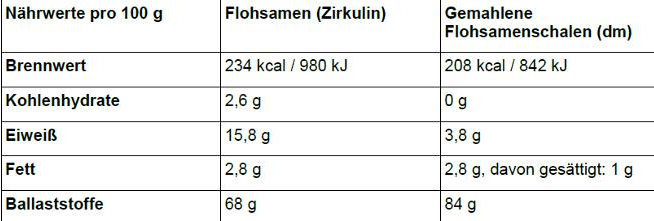
\includegraphics[width=0.8\textwidth]{test-resultaten/19/original.png}
    \caption{Origineel document.}
\end{figure}

\begin{figure}[H]
    \centering
    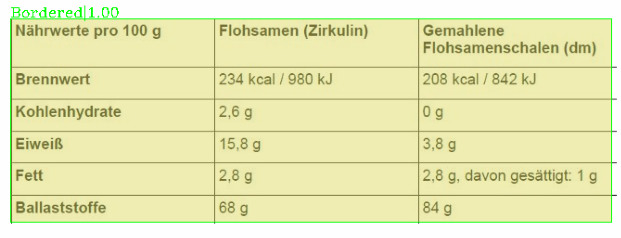
\includegraphics[width=0.8\textwidth]{test-resultaten/19/detected_tables.png}
    \caption{Gedetecteerde tabellen.}
\end{figure}

Getransformeerde tabellen met algoritme A:

\begin{tabular}{lll}
\toprule
{} &      Brennwert & 234 kcal / 980 kJ \\
\midrule
0 &  Kohlenhydrate &              2,69 \\
1 &      Eiweif\&BQ &             15,89 \\
2 &           Fett &              28 9 \\
\bottomrule
\end{tabular}

Getransformeerde tabellen met algoritme B:

\begin{tabular}{llll}
\toprule
{} & Nahrwerte pro 100 9 & Flohsamen (Zirkulin) & Gemahlene Flohsamenschalen (dm) \\
\midrule
0 &           Brennwert &    234 keal / 980 kd &               208 keal / 842 kJ \\
1 &       Kohlenhydrate &                  264 &                              og \\
2 &              EiweiB &                15,84 &                             389 \\
3 &                Fett &                  289 &     2.8 g. davon gesattigt: 1.9 \\
4 &       Ballaststoffe &                  68g &                             Bag \\
\bottomrule
\end{tabular}
\section{Document 20}

\begin{figure}[H]
    \centering
    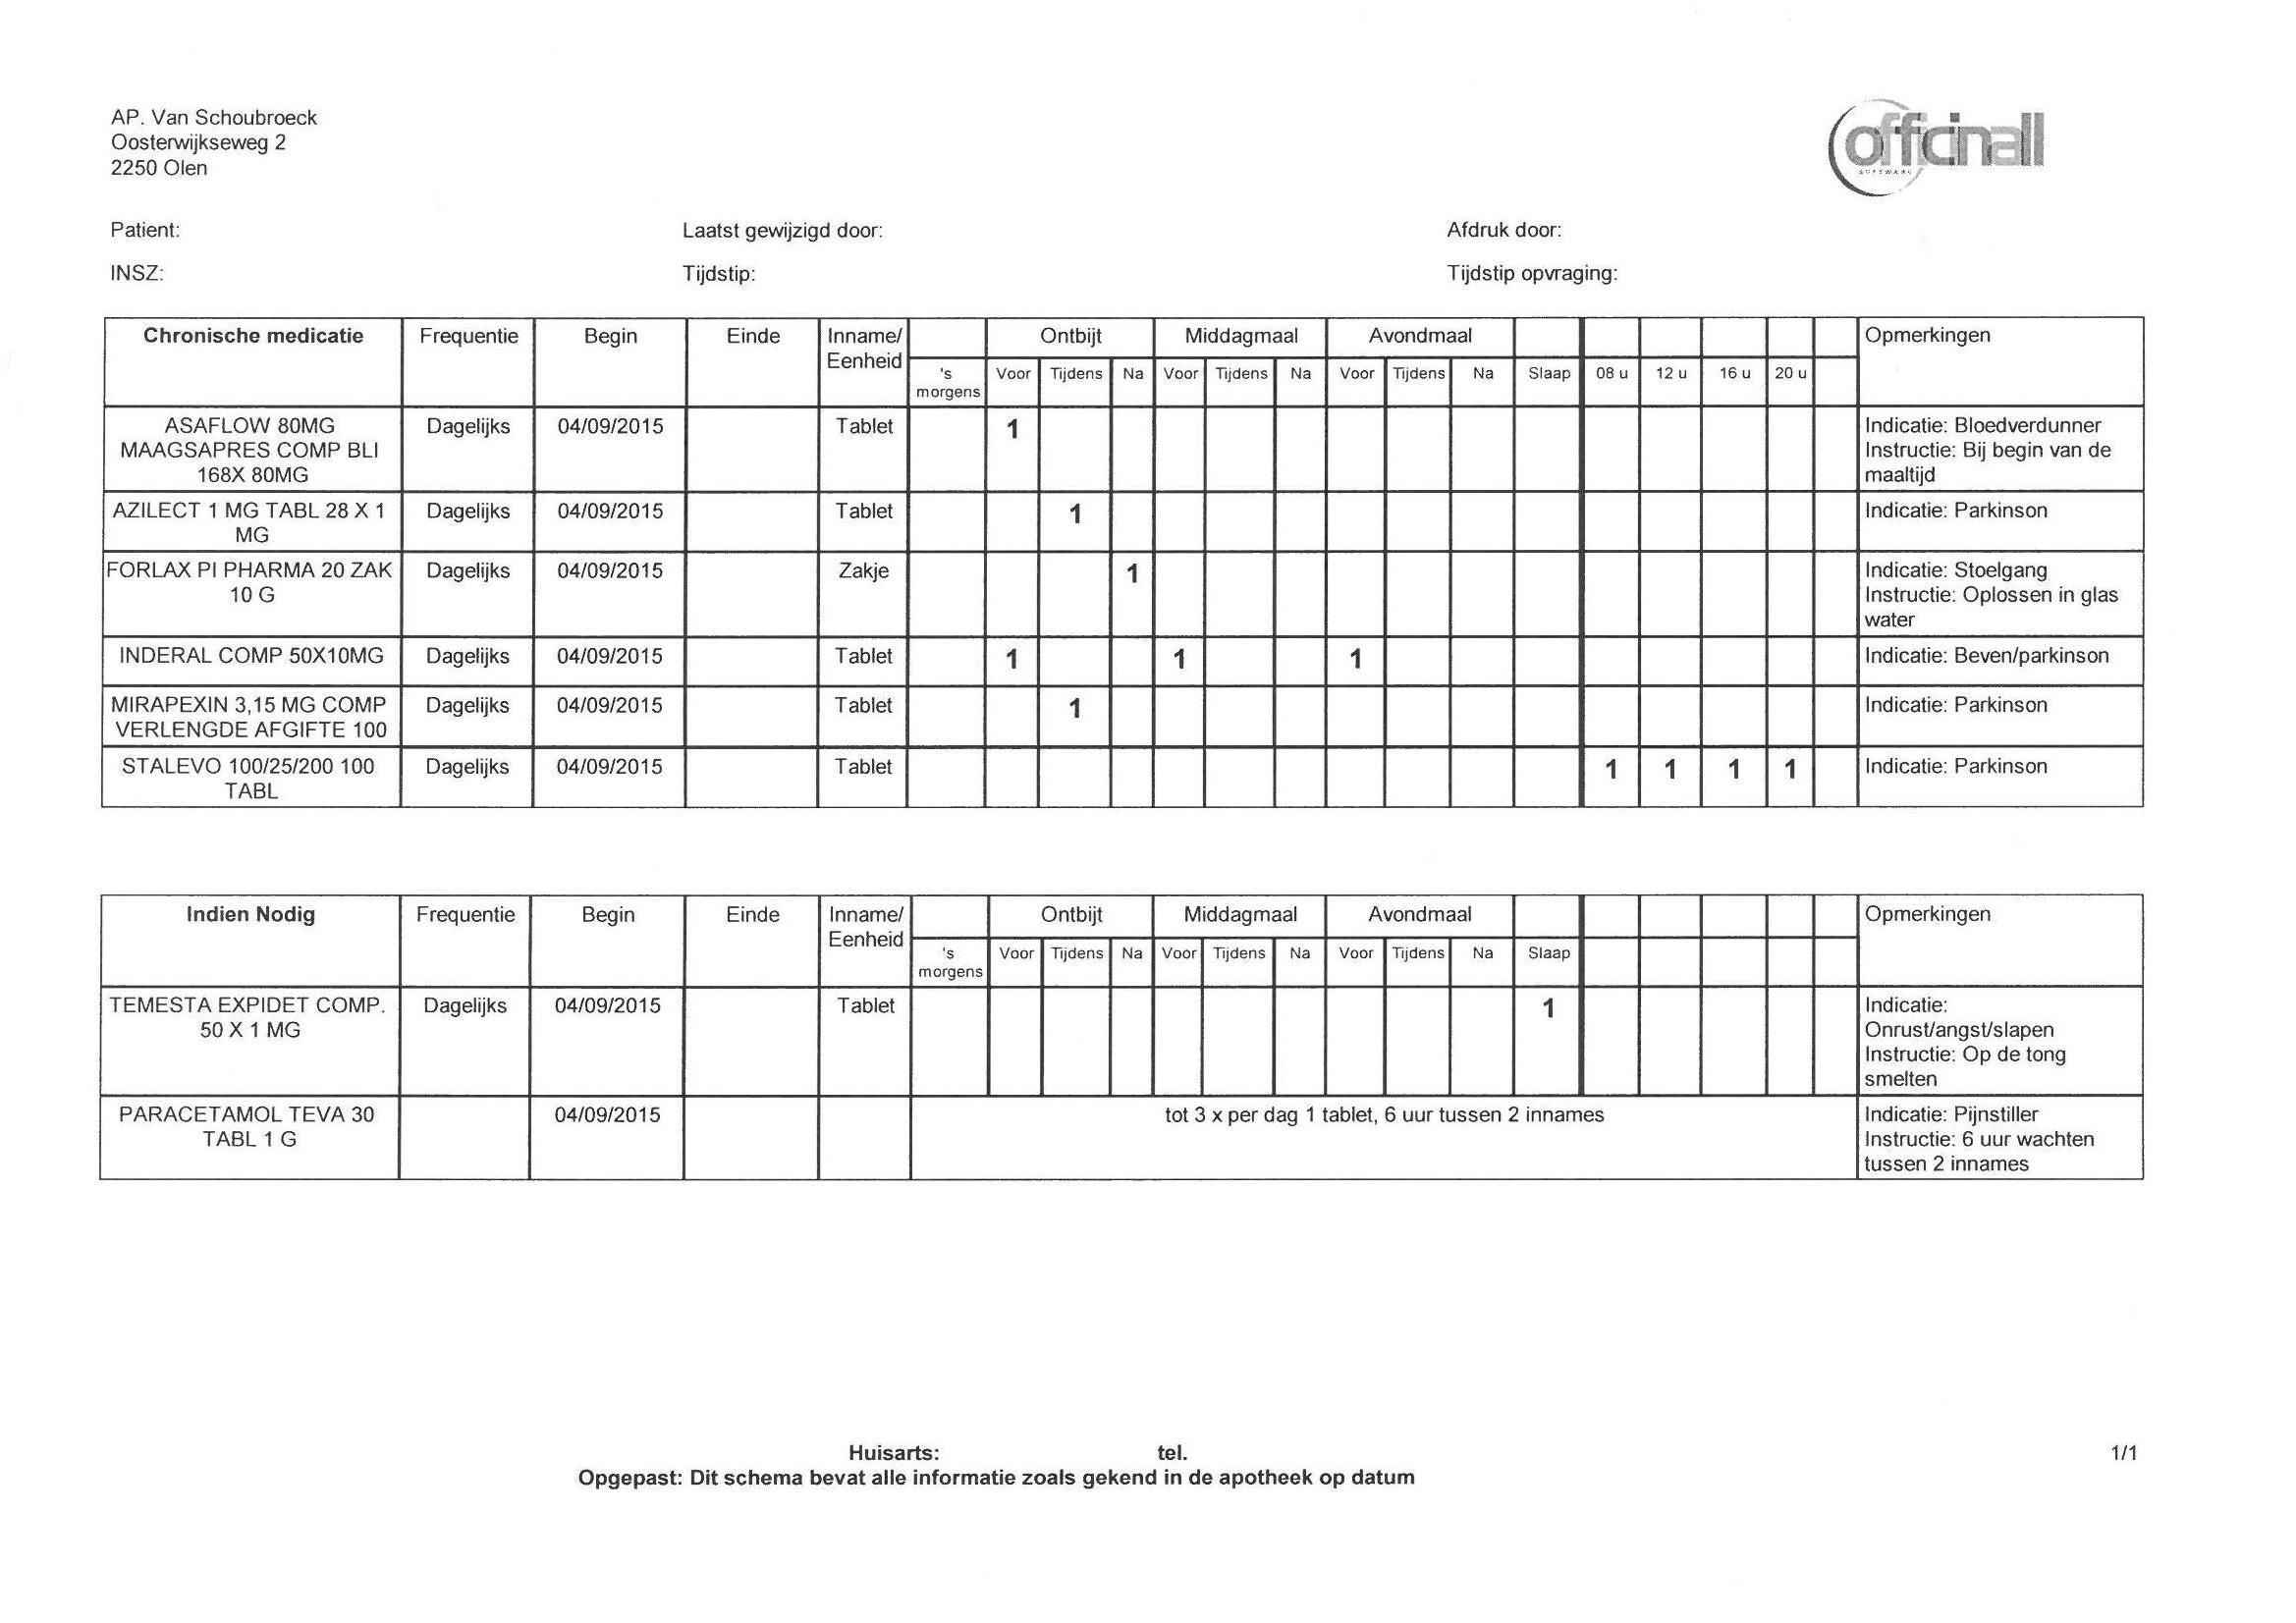
\includegraphics[width=0.8\textwidth]{test-resultaten/20/original.png}
    \caption{Origineel document.}
\end{figure}

\begin{figure}[H]
    \centering
    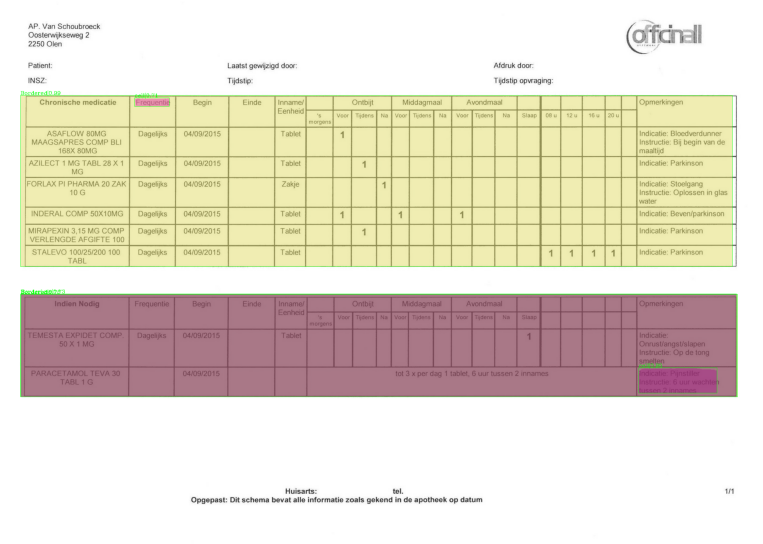
\includegraphics[width=0.8\textwidth]{test-resultaten/20/detected_tables.png}
    \caption{Gedetecteerde tabellen.}
\end{figure}

Getransformeerde tabellen met algoritme A:

Tabeltransformatie gefaald.

Getransformeerde tabellen met algoritme B:

\begin{tabular}{lllll}
\toprule
{} &                          Chronische medicatie &   Frequentie &           NaN &                                        Opmerkingen \\
\midrule
2 &    ASAFLOW 80MG MAAGSAPRES COMP BLI 168X 80MG &    Dagelijks &    04/09/2015 &  Indicatie: Bloedverdunner Instructie: Bij begi... \\
3 &                   AZILECT 1 MG TABL 28 X 1 MG &    Dagelijks &    04/09/2015 &                               Indicatie: Parkinson \\
4 &                   FORLAX PI PHARMA 20 ZAK 10G &  | Dagelijks &    04/09/2015 &  Indicatie: Stoelgang Instructie: Oplossen in glas \\
5 &                          INDERAL COMP 50X10MG &         None &    04/09/2015 &                         Indicatie: Beven/parkinson \\
6 &  MIRAPEXIN 3,15 MG COMP VERLENGDE AFGIFTE 100 &   | Dageliks &  | 04/09/2015 &                               Indicatie: Parkinson \\
7 &                   STALEVO 100/25/200 100 TABL &   | Dageliks &  | 04/09/2015 &                               Indicatie: Parkinson \\
\bottomrule
\end{tabular}
\section{Document 21}

\begin{figure}[H]
    \centering
    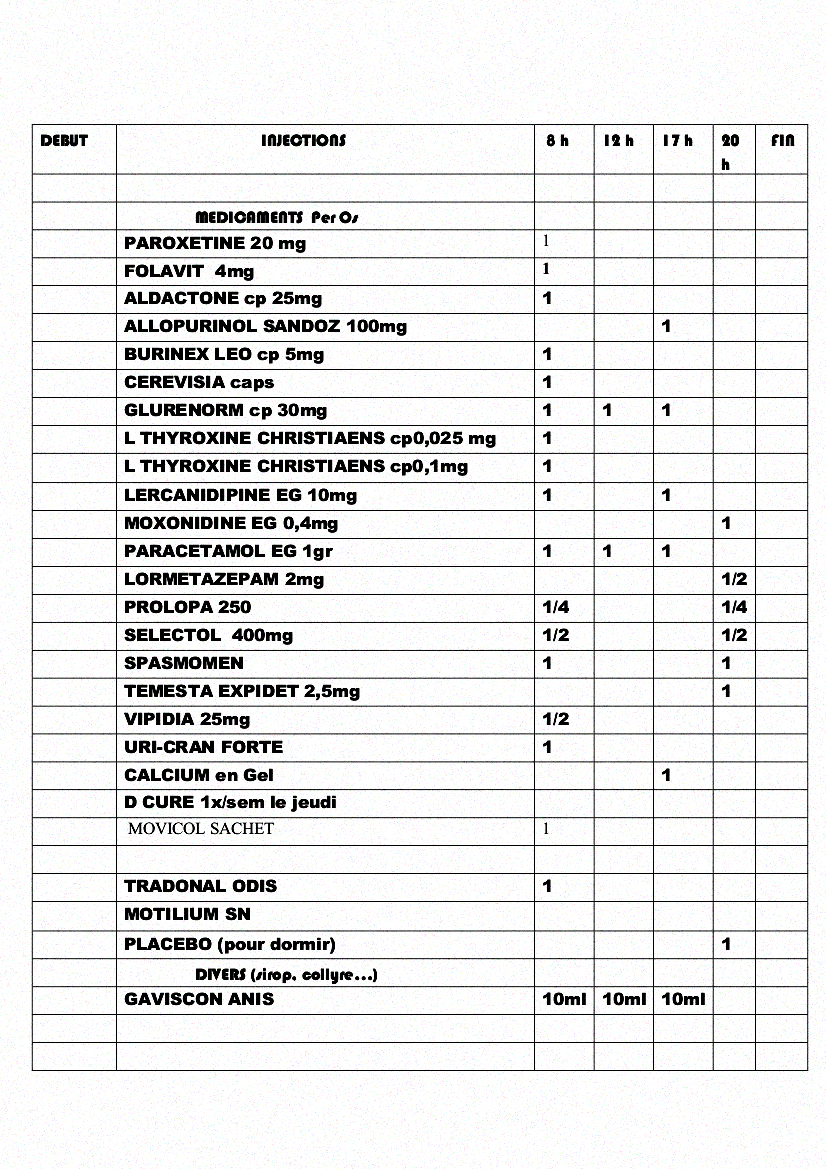
\includegraphics[width=0.8\textwidth]{test-resultaten/21/original.png}
    \caption{Origineel document.}
\end{figure}

\begin{figure}[H]
    \centering
    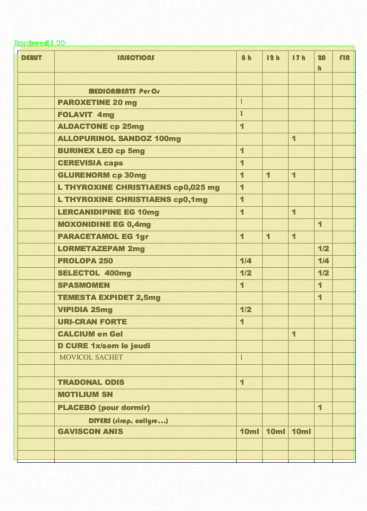
\includegraphics[width=0.8\textwidth]{test-resultaten/21/detected_tables.png}
    \caption{Gedetecteerde tabellen.}
\end{figure}

Getransformeerde tabellen met algoritme A:

Tabeltransformatie gefaald.

Getransformeerde tabellen met algoritme B:

\begin{tabular}{llllll}
\toprule
{} &                           ineotions &     8h &   ith &       | &  | oo \\
\midrule
1  &                  MEDICAMENTS Per Os &   None &  None &    None &  None \\
2  &                    PAROXETINE 20 mg &      1 &  None &    None &  None \\
3  &                         FOLAVIT 4mg &      1 &  None &    None &  None \\
4  &                   ALDACTONE cp 25mg &      = &  None &    None &  None \\
5  &            ALLOPURINOL SANDOZ 100mg &   None &  None &       4 &  None \\
6  &                  BURINEX LEO cp 5mg &   None &  None &    None &  None \\
7  &                      CEREVISIA caps &   None &  None &    None &  None \\
8  &                   GLURENORM cp 30mg &   None &  None &    None &  None \\
9  &  L THYROXINE CHRISTIAENS cp0,025 mg &   None &  None &    None &  None \\
10 &     L THYROXINE CHRISTIAENS cp0,1mg &   None &  None &    None &  None \\
11 &               LERCANIDIPINE EG 10mg &     3] &  None &    None &  None \\
12 &                 MOXONIDINE EG 0,4mg &   None &  None &    None &    41 \\
13 &                  PARACETAMOL EG 1gr &      1 &    41 &      41 &  None \\
14 &                    LORMETAZEPAM 2mg &   None &  None &    None &   112 \\
15 &                         PROLOPA 250 &     4a &  None &    None &    14 \\
16 &                      SELECTOL 400mg &     12 &  None &    None &    12 \\
17 &                           SPASMOMEN &     41 &  None &    None &    41 \\
18 &               TEMESTA EXPIDET 2,5mg &   None &  None &    None &    41 \\
19 &                        VIPIDIA 25mg &    412 &  None &    None &  None \\
20 &                      URI-CRAN FORTE &     41 &  None &    None &  None \\
21 &                      CALCIUM en Gel &   None &  None &      41 &  None \\
22 &              D CURE 1x/sem le jeudi &   None &  None &    None &  None \\
23 &                      MOVICOL SACHET &      1 &  None &    None &  None \\
25 &                       TRADONAL ODIS &     41 &  None &    None &  None \\
26 &                         MOTILIUM SN &   None &  None &    None &  None \\
27 &               PLACEBO (pour dormir) &   None &  None &    None &     4 \\
28 &          DIVERS (sirop, collyre...) &   None &  None &    None &  None \\
29 &                       GAVISCON ANIS &  410ml &     | &  | 10m1 &  None \\
\bottomrule
\end{tabular}
\section{Document 22}

\begin{figure}[H]
    \centering
    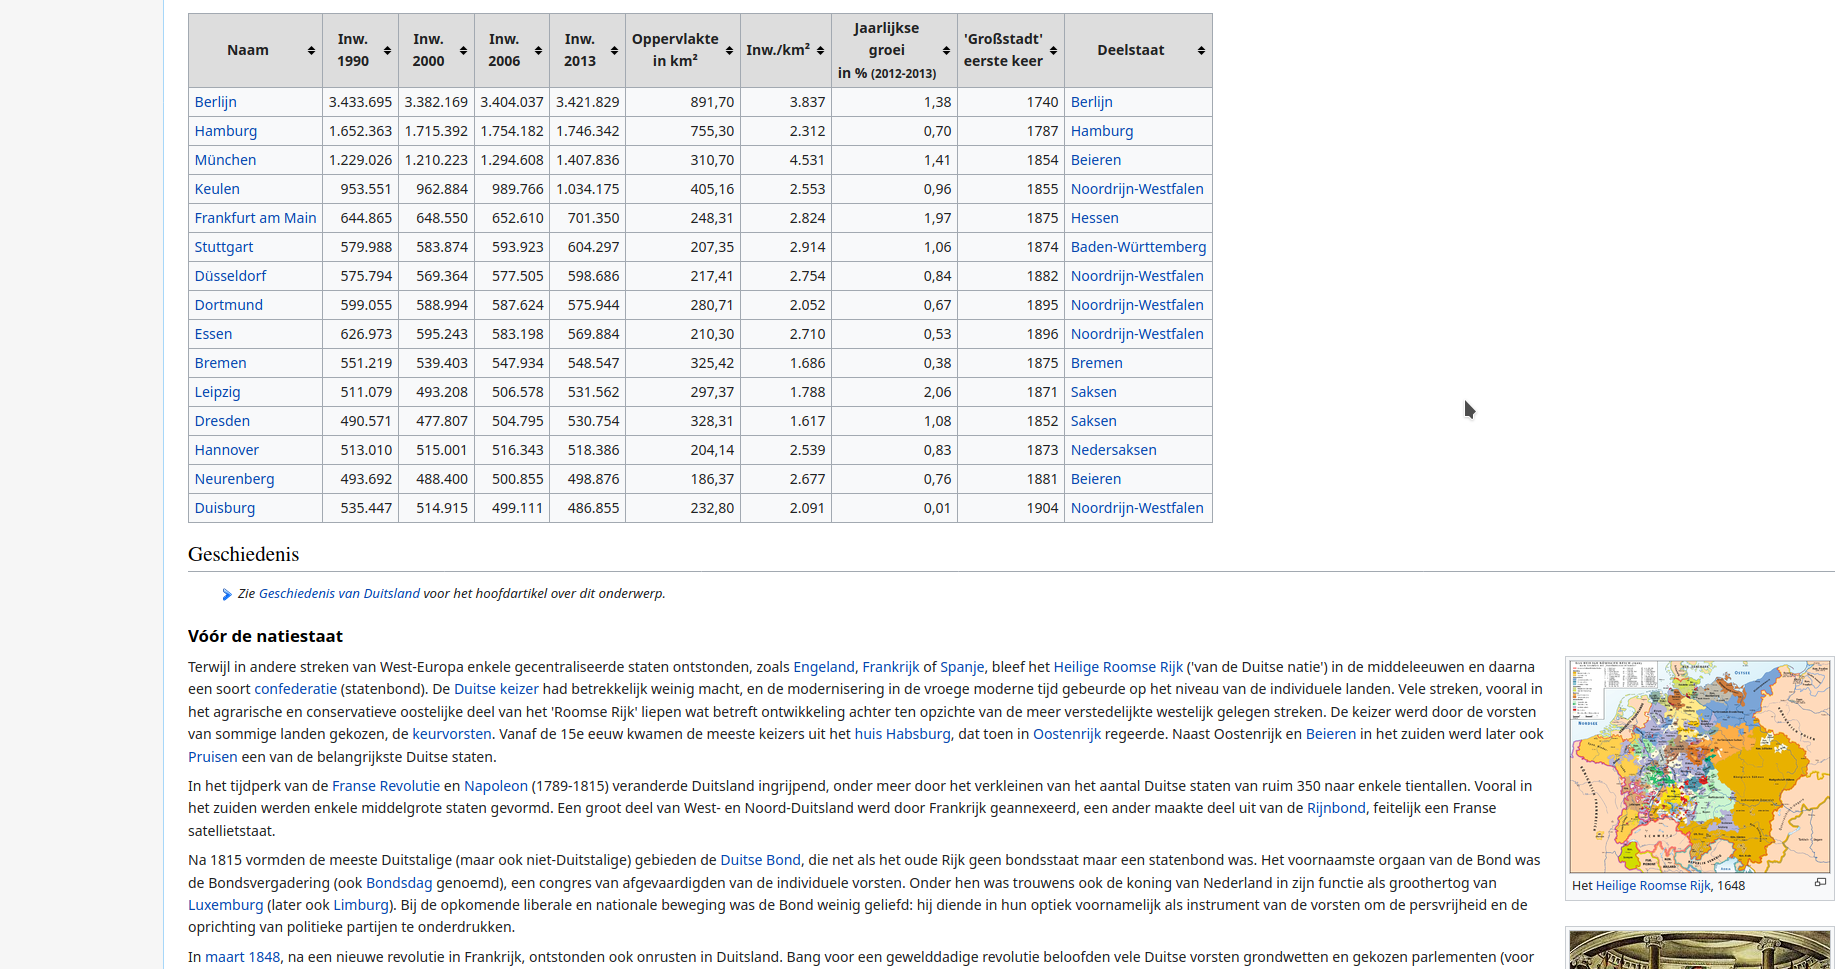
\includegraphics[width=0.8\textwidth]{test-resultaten/22/original.png}
    \caption{Origineel document.}
\end{figure}

\begin{figure}[H]
    \centering
    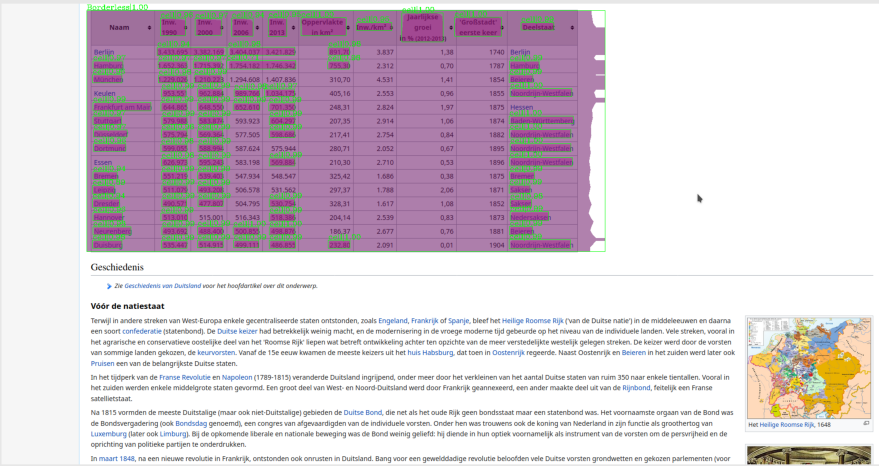
\includegraphics[width=0.8\textwidth]{test-resultaten/22/detected_tables.png}
    \caption{Gedetecteerde tabellen.}
\end{figure}

Getransformeerde tabellen met algoritme A:

Tabeltransformatie gefaald.

Getransformeerde tabellen met algoritme B:

\begin{tabular}{llllllllll}
\toprule
{} & Jaarlijkse gro) «| &             Naam =e & | 2 | 1990 &         2000 &    Inw. 2006 &  Inw. | 2013 & Opperviakte | | in km™ & sum? « &      Deelstaat | erste keer \\
\midrule
0  &               1,38 &             Berlijn &  3.433.695 &  | 3.382.169 &  | 3.404.037 &  | 3.421.829 &                 891,70 &  3.837 &              1749 | Berliin \\
1  &               0,70 &             Hamburg &  1.652.363 &  | 1.715.392 &  | 1.754.182 &  | 1.746.342 &                 755,30 &   2312 &              1787 | Hamburg \\
2  &               1,41 &            Miinchen &  1,229,026 &  | 1.210.223 &  | 1.294.608 &  | 1.407.836 &                 310,70 &  4.531 &              1854 | Beieren \\
3  &               0,96 &              Keulen &   953.551] &     962.884] &     989.766] &    1.034.175 &                 405,16 &  2.553 &  1855 | Noordrijn-Westfalen \\
4  &               1,97 &  Frankfurt am Main| &   644.865] &      648.550 &     652.610] &      701.350 &                 248,31 &   2824 &               1875 | Hessen \\
5  &               1,06 &           Stuttgart &       None &     583.874] &     593.923] &      604.297 &                 207,35 &   2914 &   1874 | Baden-Wiirttemberg \\
6  &               0,84 &          Dusseldorf &       None &     569.364] &     577.505) &      598.686 &                 217,41 &   2754 &  1882 | Noordrijn-Westfalen \\
7  &               0,67 &            Dortmund &   599.055] &     588.994] &     587.624) &      575.944 &                 280,71 &  2.052 &  1895 | Noordrijn-Westfalen \\
8  &               0,53 &               Essen &   626.973] &     595.243] &     583.198] &      569.884 &                 210,30 &  2.710 &  1896 | Noordrijn-Westfalen \\
9  &               0,38 &              Bremen &   551.219] &     539.403] &     547.934) &      548.547 &                 325,42 &  1.686 &               1875 | Bremen \\
10 &               2,06 &             Leipzig &   511,079] &     493.208] &     506.578) &      531.562 &                 297,37 &  1.788 &               1871 | Saksen \\
11 &               1,08 &             Dresden &   490.571] &     477.807| &     504.795] &      530.754 &                 328,31 &  1.617 &               1852 | Saksen \\
12 &               0,83 &            Hannover &   513.010| &     515.001] &     516.343) &      518.386 &                 204,14 &  2.539 &          1873 | Nedersaksen \\
13 &               0,76 &          Neurenberg &    493,692 &     488.400] &     500.855) &      498.876 &                 186,37 &  2.677 &              1881 | Beieren \\
14 &               0,01 &            Duisburg &       None &     514.915| &     499.111] &     486.855. &                 232,80 &  2.091 &   1904. Noordrijn-Westfalen \\
\bottomrule
\end{tabular}
\section{Document 23}

\begin{figure}[H]
    \centering
    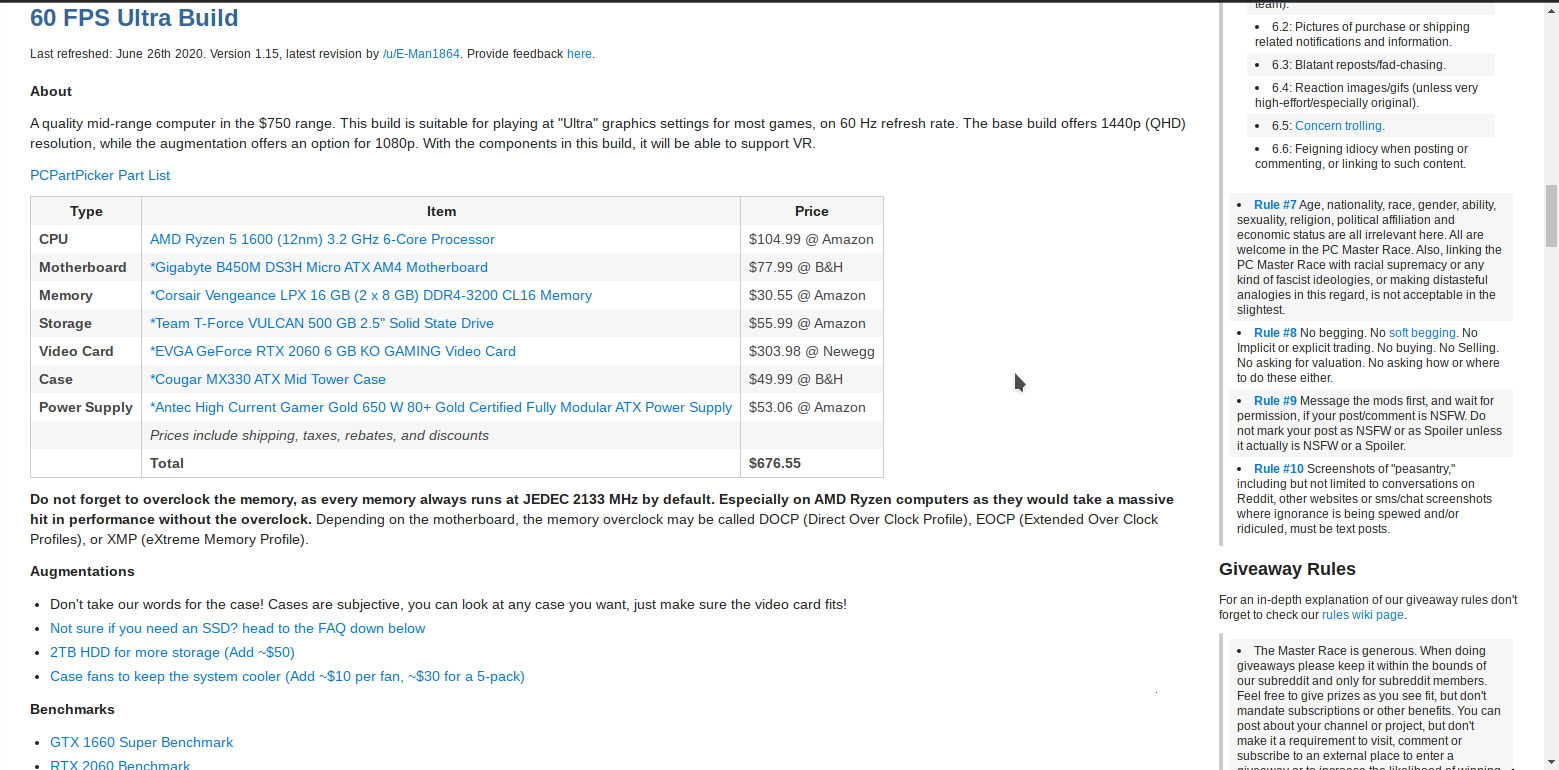
\includegraphics[width=0.8\textwidth]{test-resultaten/23/original.png}
    \caption{Origineel document.}
\end{figure}

\begin{figure}[H]
    \centering
    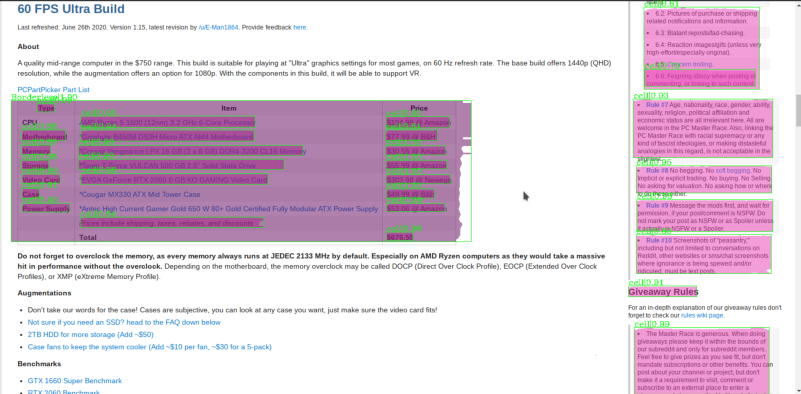
\includegraphics[width=0.8\textwidth]{test-resultaten/23/detected_tables.png}
    \caption{Gedetecteerde tabellen.}
\end{figure}

Getransformeerde tabellen met algoritme A:

\begin{tabular}{llll}
\toprule
{} &          Type &                                               Item &             Price \\
\midrule
0 &           CPU &   AMD Ryzen 5 1600 (12nm) 3.2 GHz 6-Core Processor &  \$104.99 @ Amazon \\
1 &   Motherboard &     “Gigabyte B450M DS3H Micro ATX AM4 Motherboard &      \$77.99 @ B\&H \\
2 &        Memory &  “Corsair Vengeance LPX 16 GB (2 x 8 GB) DDR4-3... &   \$30.55 @ Amazon \\
3 &       Storage &  *Team T-Force VULCAN 500 GB 2.5" Solid State D... &   \$55.99 @ Amazon \\
4 &    Video Card &   *EVGA GeForce RTX 2060 6 GB KO GAMING Video Card &  \$303.98 @ Newegg \\
5 &          Case &                   “Cougar MX330 ATX Mid Tower Case &      \$49.99 @ B\&H \\
6 &  Power Supply &                                    \$53 06 @ Amazo! &              None \\
7 &         Total &                                            \$676.55 &              None \\
\bottomrule
\end{tabular}

Getransformeerde tabellen met algoritme B:

\begin{tabular}{llll}
\toprule
{} &          Type &                                               Item &             Price \\
\midrule
0 &           cPU &   AMD Ryzen 5 1600 (12nm) 3.2 GHz 6-Core Processor &  \$104.99 @ Amazon \\
1 &   Motherboard &     *Gigabyte B450M DS3H Micro ATX AM4 Motherboard &      \$77.99 @ B\&H \\
2 &        Memory &  “Corsair Vengeance LPX 16 GB (2 x 8 GB) DDR4-3... &   \$30.55 @ Amazon \\
3 &       Storage &  “Team T-Force VULCAN 500 GB 2.5” Solid State D... &   \$55.99 @ Amazon \\
4 &    Video Card &   “EVGA GeForce RTX 2060 6 GB KO GAMING Video Card &  \$303.98 @ Newegg \\
5 &          Case &                   *Cougar MX330 ATX Mid Tower Case &      \$49.99 @ B\&H \\
6 &  Power Supply &  *Antec High Current Gamer Gold 650 W 80+ Gold ... &   \$53.06 @ Amazon \\
7 &          None &  Prices include shipping, taxes, rebates, and d... &              None \\
8 &          None &                                              Total &           \$676.55 \\
\bottomrule
\end{tabular}
\section{Document 24}

\begin{figure}[H]
    \centering
    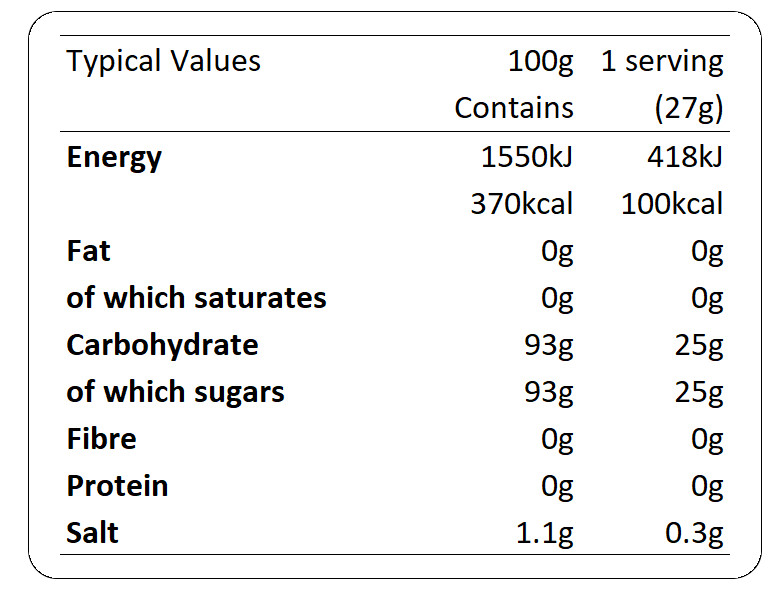
\includegraphics[width=0.8\textwidth]{test-resultaten/24/original.jpg}
    \caption{Origineel document.}
\end{figure}

\begin{figure}[H]
    \centering
    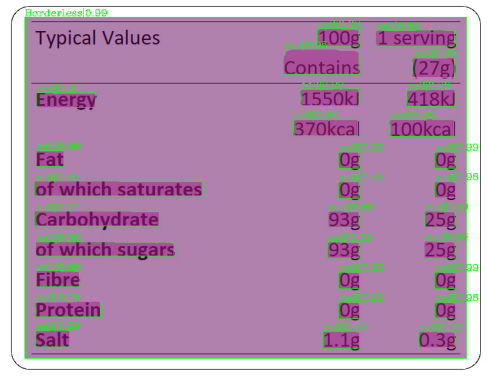
\includegraphics[width=0.8\textwidth]{test-resultaten/24/detected_tables.png}
    \caption{Gedetecteerde tabellen.}
\end{figure}

Getransformeerde tabellen met algoritme A:

Getransformeerde tabellen met algoritme B:
\section{Document 25}

\begin{figure}[H]
    \centering
    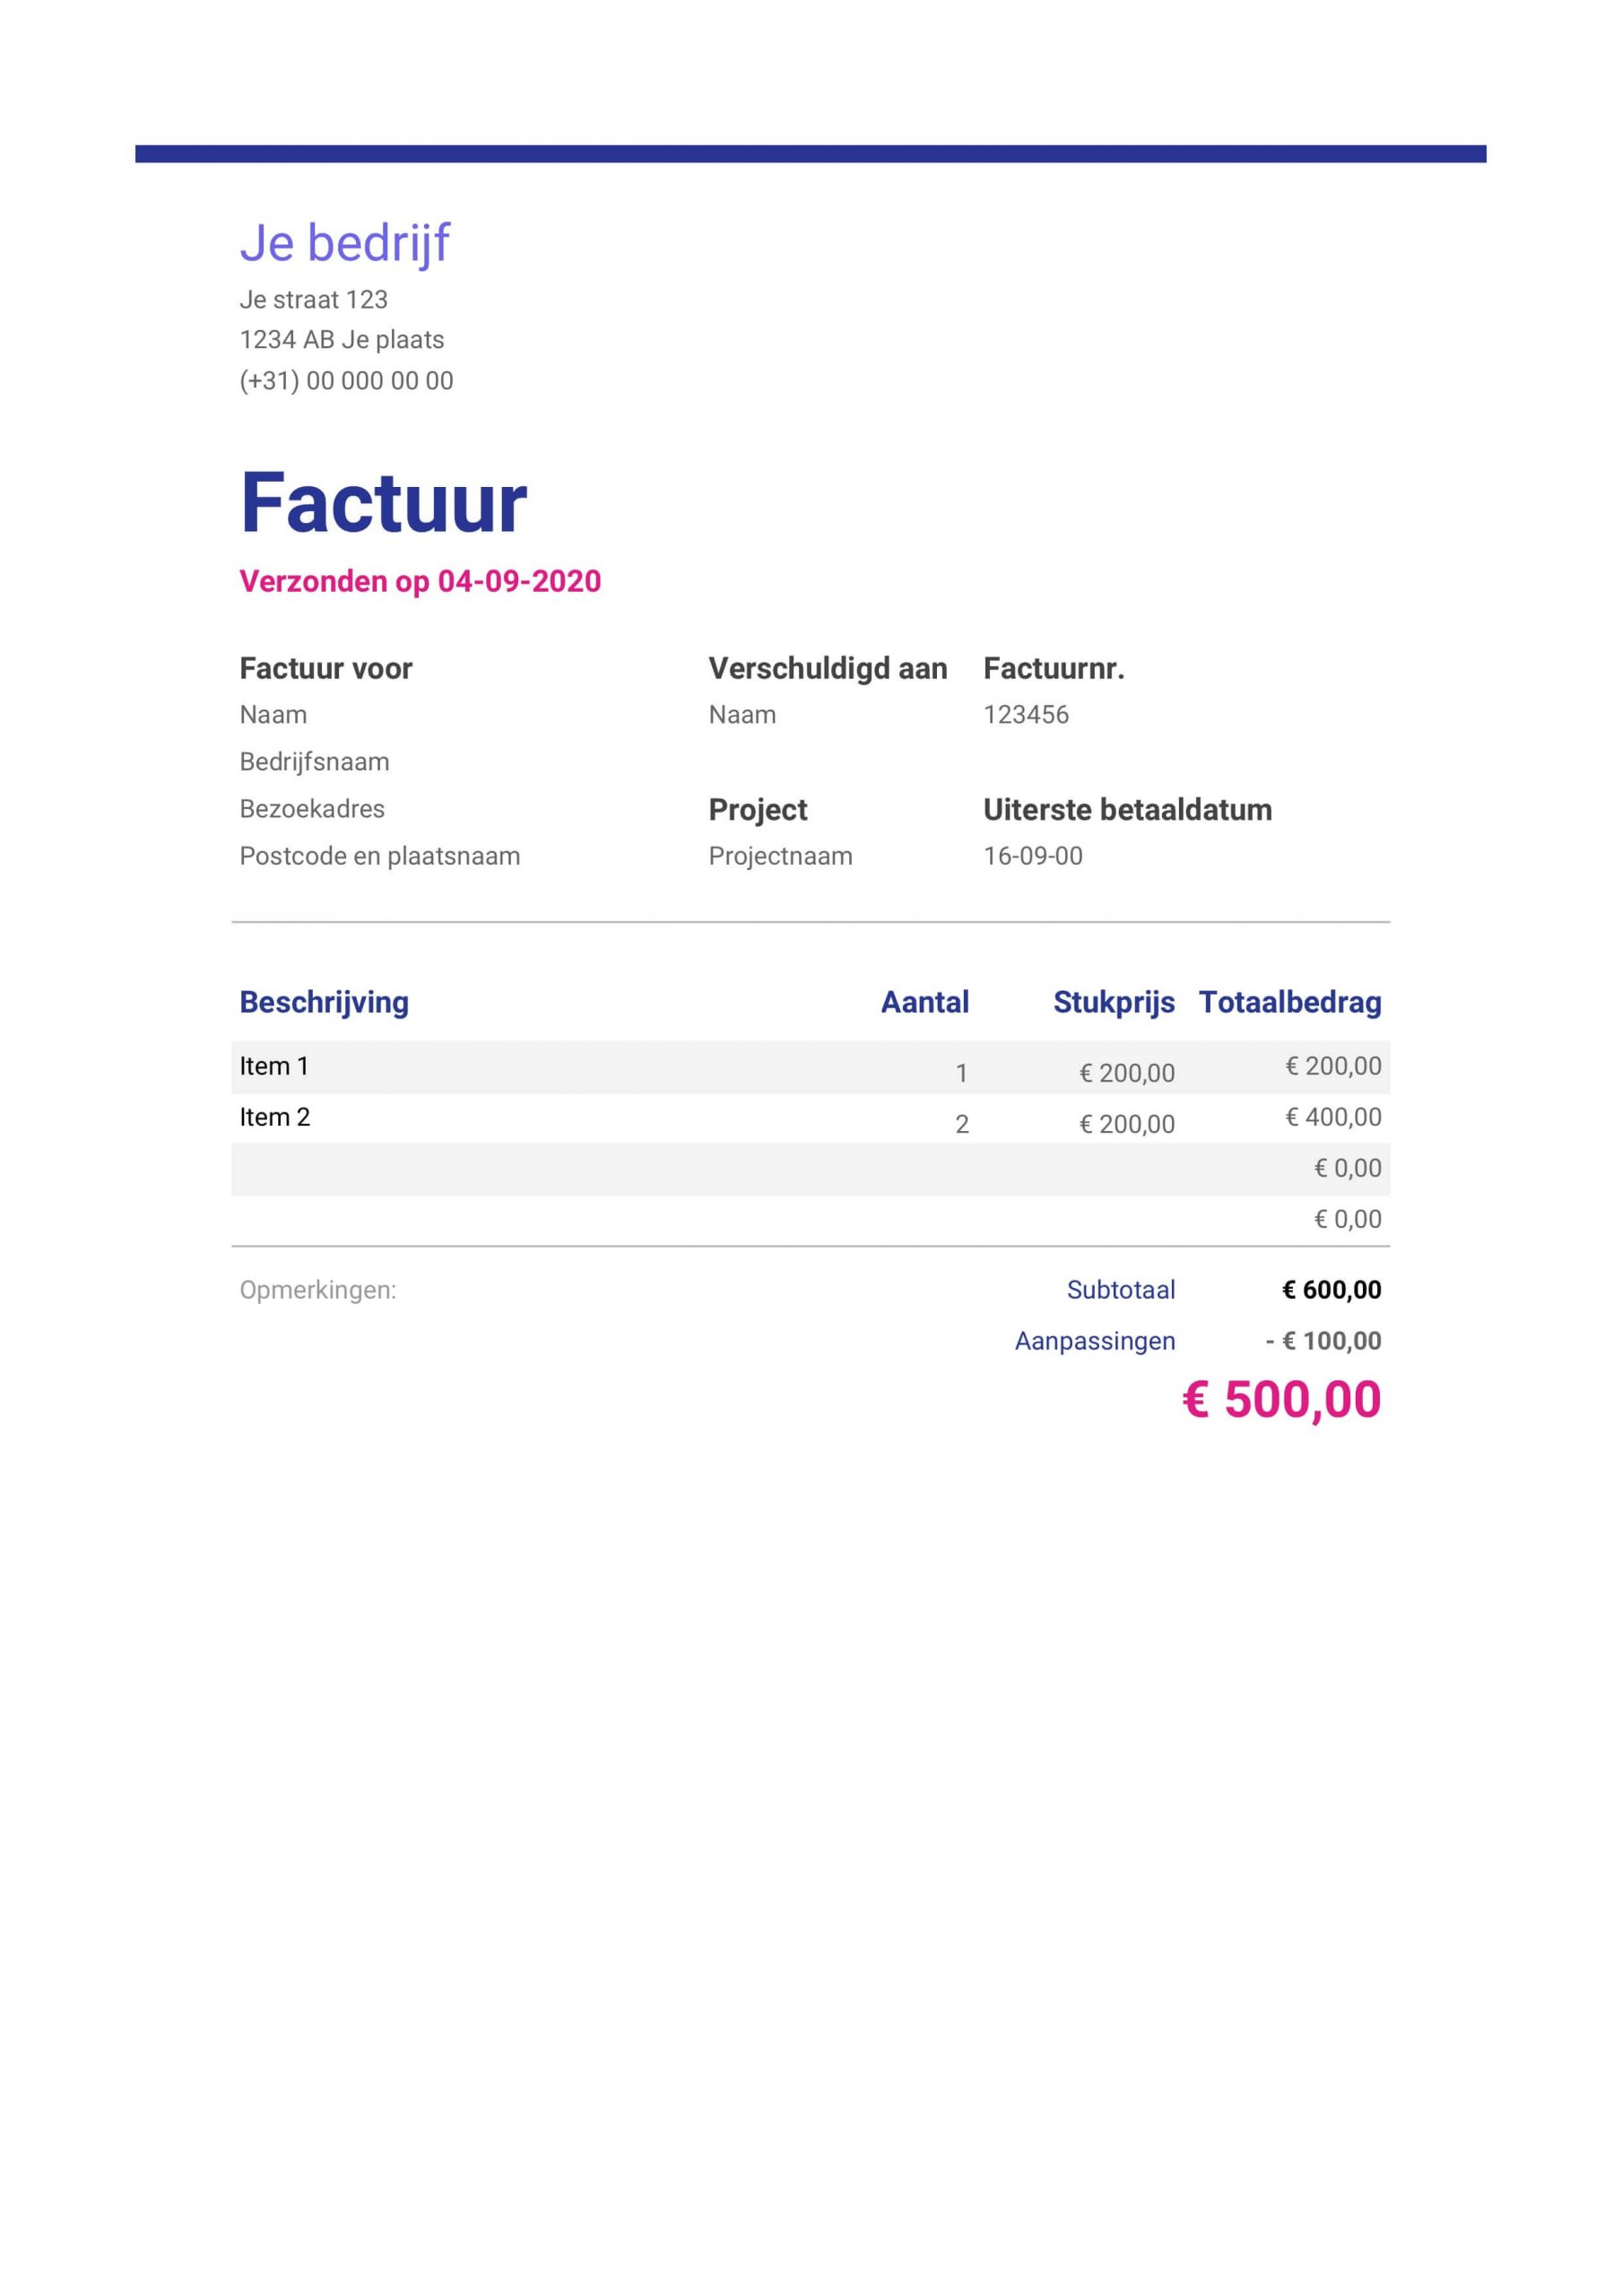
\includegraphics[width=0.8\textwidth]{test-resultaten/25/original.jpg}
    \caption{Origineel document.}
\end{figure}

\begin{figure}[H]
    \centering
    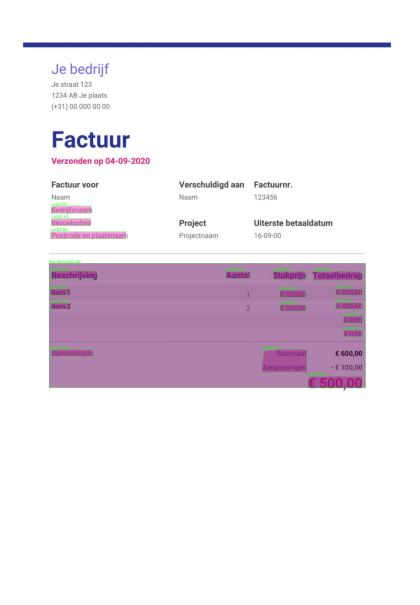
\includegraphics[width=0.8\textwidth]{test-resultaten/25/detected_tables.png}
    \caption{Gedetecteerde tabellen.}
\end{figure}

Getransformeerde tabellen met algoritme A:

\begin{tabular}{llll}
\toprule
{} &  Beschriivina &                   Aantal &                   T \\
\midrule
0 &        Item 1 &                 € 200.0C &            € 200,00 \\
1 &        Item 2 &                  € 20000 &            € 400,00 \\
2 &        € 0,00 &                     None &                None \\
3 &         €0,00 &                     None &                None \\
4 &  Opmerkingen: &  Subtotaal\textbackslash nAanpassingen &  € 600,00\textbackslash n€ 100,00 \\
5 &      € 500 00 &                     None &                None \\
\bottomrule
\end{tabular}

Getransformeerde tabellen met algoritme B:

\begin{tabular}{llllll}
\toprule
{} &  Beschrijving & Aantal &     Stukprijs & Totaalbedrag &   NaN \\
\midrule
0 &        Item 1 &      1 &      € 200,00 &     € 200,00 &  None \\
1 &        Item 2 &      2 &      € 200,00 &     € 400,00 &  None \\
2 &  Opmerkingen: &   None &     Subtotaal &     € 600,00 &  None \\
3 &          None &   None &          None &       € 0,00 &  None \\
4 &          None &   None &          None &       € 0,00 &  None \\
5 &          None &   None &  Aanpassingen &   - € 100,00 &  None \\
6 &          None &   None &          None &       500 00 &     € \\
\bottomrule
\end{tabular}
\section{Document 26}

\begin{figure}[H]
    \centering
    \includegraphics[width=0.8\textwidth]{test-resultaten/26/original.jpg}
    \caption{Origineel document.}
\end{figure}

\begin{figure}[H]
    \centering
    \includegraphics[width=0.8\textwidth]{test-resultaten/26/detected_tables.png}
    \caption{Gedetecteerde tabellen.}
\end{figure}

Getransformeerde tabellen met algoritme A:

\begin{tabular}{lllll}
\toprule
{} &        Field & Dislike & Neutral & Like \\
\midrule
0 &    Pistachio &      Qo &      13 &    4 \\
1 &      Vanilla &      13 &       6 &    7 \\
2 &  ‘Strawberry &      10 &      10 &    6 \\
\bottomrule
\end{tabular}

Getransformeerde tabellen met algoritme B:

\begin{tabular}{lllll}
\toprule
{} &       Field & Dislike & Neutral & Like \\
\midrule
0 &   Pistachio &       9 &      33 &    4 \\
1 &     Vanilla &      13 &       6 &    7 \\
2 &  Strawberry &      10 &      10 &    6 \\
\bottomrule
\end{tabular}
\section{Document 27}

\begin{figure}[H]
    \centering
    \includegraphics[width=0.8\textwidth]{test-resultaten/27/original.png}
    \caption{Origineel document.}
\end{figure}

\begin{figure}[H]
    \centering
    \includegraphics[width=0.8\textwidth]{test-resultaten/27/detected_tables.png}
    \caption{Gedetecteerde tabellen.}
\end{figure}

Getransformeerde tabellen met algoritme A:

Tabeltransformatie gefaald.

Getransformeerde tabellen met algoritme B:

\begin{tabular}{lll}
\toprule
{} &                        NaN & Concentration \\
\midrule
0  &  Compound Protein (g/100g) &            13 \\
1  &               Fat (g/100g) &           0.2 \\
2  &      Carbohydrate (g/100g) &            71 \\
3  &                      Fibre &           2.1 \\
4  &           (g/100g) Vitamin &          None \\
5  &        Vitamin C (mg/100g) &            70 \\
6  &          Vitamin (mg/100g) &          0.14 \\
7  &                  E Mineral &          None \\
8  &        Potassium (mg/100g) &           170 \\
9  &          Calcium (mg/100g) &            25 \\
10 &        Magnesium (mg/100g) &            10 \\
11 &       Phosphorus (mg/100g) &            33 \\
12 &                     Sulfur &            50 \\
13 &             Tron (mg/100g) &            03 \\
\bottomrule
\end{tabular}
\section{Document 28}

\begin{figure}[H]
    \centering
    \includegraphics[width=0.8\textwidth]{test-resultaten/28/original.png}
    \caption{Origineel document.}
\end{figure}

\begin{figure}[H]
    \centering
    \includegraphics[width=0.8\textwidth]{test-resultaten/28/detected_tables.png}
    \caption{Gedetecteerde tabellen.}
\end{figure}

Getransformeerde tabellen met algoritme A:

\begin{tabular}{lll}
\toprule
{} &                              Foutmelding &  33.8 \\
\midrule
0 &                   Parkeerpagina websites &  27,4 \\
1 &                          Bedrijfswebsite &  14,6 \\
2 &  Parkeerpagina niet-commerciéle websites &  13,0 \\
3 &                 Niet-commerciéle website &   6,6 \\
4 &                   Website om te verkopen &   2,8 \\
5 &                  Persoonlijke/gezinsblog &   1,4 \\
6 &                            Pay-per-click &   0,2 \\
7 &                             Portal/media &   0,2 \\
8 &                        Bron: DNS Belgium &  None \\
\bottomrule
\end{tabular}

\begin{tabular}{lllll}
\toprule
{} &          Bedrijfswebsite &  48.0 &  54.7 & Verandering\textbackslash n6,7 \\
\midrule
0 &    Niet-commerciéle web- &  18,6 &  18,3 &             -0,3 \\
1 &              Foutmelding &  15,4 &  16,1 &              0,7 \\
2 &            Pay per click &   2,1 &   0,7 &              1,4 \\
3 &  Persoonlijke/gezinsblog &    48 &   3,2 &              1,6 \\
4 &                  Webshop &   3,8 &   2,1 &              1,7 \\
5 &            Portaal/media &   1,7 &   0,7 &              1,0 \\
6 &   Website om te verkopen &   2,3 &   2,5 &              0,2 \\
7 &                   Andere &   3,3 &   1,8 &              1,5 \\
\bottomrule
\end{tabular}

\begin{tabular}{lll}
\toprule
{} &                   Parkeerpagina websites &  26.4 \\
\midrule
0 &                              Foutmelding &  29,7 \\
1 &                          Bedrijfswebsite &  13,6 \\
2 &  Parkeerpagina niet-commerciéle websites &  11,0 \\
3 &                 Niet-commerciéle website &   6,6 \\
4 &                   Website om te verkopen &   1,0 \\
5 &                            Pay-per-click &   0,8 \\
6 &                  Persoonlijke/gezinsblog &   0,8 \\
7 &                             Portal/media &   0,2 \\
\bottomrule
\end{tabular}

Getransformeerde tabellen met algoritme B:

\begin{tabular}{lllll}
\toprule
{} &          HMM Vall &    oN &                      NaN &       NaN \\
\midrule
0 &              None &  33,8 &              Foutmelding &      None \\
1 &          websites &  27,4 &            Parkeerpagina &      None \\
2 &              None &  14,6 &          Bedrijfswebsite &      None \\
3 &  niet-commerciéle &  13,0 &            Parkeerpagina &  websites \\
4 &           website &   6,6 &         Niet-commerciéle &      None \\
5 &          verkopen &   2,8 &            Website om te &      None \\
6 &              None &   1,4 &  Persoonlijke/gezinsblog &      None \\
7 &              None &   0,2 &            Pay-per-click &      None \\
8 &              None &   0,2 &             Portal/media &      None \\
\bottomrule
\end{tabular}

\begin{tabular}{llllll}
\toprule
{} & verandering &                      NaN &   NaN &   NaN &       NaN \\
\midrule
0 &         6,7 &          Bedrijfswebsite &  48,0 &  54,7 &      None \\
1 &        -0,3 &         Niet-commercitie &  18,6 &  18,3 &      web- \\
2 &         0,7 &              Foutmelding &  15,4 &  16,1 &      None \\
3 &        -1,4 &            Pay per click &   2,1 &   0,7 &      None \\
4 &        -1,6 &  Persoonlijke/gezinsblog &   4,8 &   3,2 &      None \\
5 &        -1,7 &                  Webshop &   3,8 &   2,1 &      None \\
6 &        -1,0 &            Portaal/media &   1,7 &   0,7 &      None \\
7 &         0,2 &            Website om te &   2,3 &   2,5 &  verkopen \\
8 &        -1,5 &                   Andere &   3,3 &   1,8 &      None \\
\bottomrule
\end{tabular}

\begin{tabular}{lllll}
\toprule
{} &        inhoud van & .Drussels &  culo &                      NaN \\
\midrule
0 &          websites &      None &  36,3 &            Parkeerpagina \\
1 &              None &      None &  29,7 &              Foutmelding \\
2 &              None &      None &  13,6 &          Bedrijfswebsite \\
3 &  niet-commerciéle &  websites &  11,0 &            Parkeerpagina \\
4 &           website &      None &   6,6 &         Niet-commerciéle \\
5 &          verkopen &      None &   1,0 &            Website om te \\
6 &              None &      None &   0,8 &            Pay-per-click \\
7 &              None &      None &   0,8 &  Persoonlijke/gezinsblog \\
8 &              None &      None &   0,2 &             Portal/media \\
\bottomrule
\end{tabular}
\section{Document 29}

\begin{figure}[H]
    \centering
    \includegraphics[width=0.8\textwidth]{test-resultaten/29/original.png}
    \caption{Origineel document.}
\end{figure}

\begin{figure}[H]
    \centering
    \includegraphics[width=0.8\textwidth]{test-resultaten/29/detected_tables.png}
    \caption{Gedetecteerde tabellen.}
\end{figure}

Getransformeerde tabellen met algoritme A:

Tabeltransformatie gefaald.

Getransformeerde tabellen met algoritme B:

\begin{tabular}{llllllllllllllllllllll}
\toprule
{} &           MIJN & GENEESMIDDELEN &            NaN &         NaN &       NaN &        NaN &        NaN &     NaN &     ONTBIT &   NaN &   NaN &     NaN &        NaN & MIDDAGMAAL &    NaN &     NaN &        NaN & AVONDMAAL &    NaN &      NaN &            NaN \\
\midrule
1 &  ‘Geneesmiddet &          Basis &           Yorm &  Frequentie &  | Inname &  | Eenheid &  | Nuchter &  | Voor &  |Tijdens| &    Wa &     | &  | Noor &  |Tijdens] &         Na &  | 16u &  | Voor &  |Tiidens) &        Na &  | 20u &  | Staap &  | OPMERKINGEN \\
2 &   vb. Dafa.gan &        sooma — &  | truistable: &    | 2xttag &     | cae &     table: &       None &    None &          1 &  None &  None &    None &       None &       None &   None &    None &          1 &      None &   None &     None &           None \\
\bottomrule
\end{tabular}

\section{Document 30}

\begin{figure}[H]
    \centering
    \includegraphics[width=0.8\textwidth]{test-resultaten/30/original.png}
    \caption{Origineel document.}
\end{figure}

\begin{figure}[H]
    \centering
    \includegraphics[width=0.8\textwidth]{test-resultaten/30/detected_tables.png}
    \caption{Gedetecteerde tabellen.}
\end{figure}

Getransformeerde tabellen met algoritme A:

Getransformeerde tabellen met algoritme B:
